\documentclass[12pt,a4paper,fleqn]{report}
\usepackage[left=35mm,right=25mm,top=25mm,bottom=25mm]{geometry}
\usepackage[sort&compress,square,numbers]{natbib}
\usepackage{bookmark}
\usepackage{url}
\usepackage{hyperref}
\usepackage{svg}
\hypersetup{
    colorlinks=false, %set true if you want colored links
    linktoc=all,     %set to all if you want both sections and subsections linked
    linkcolor=blue,  %choose some color if you want links to stand out
}
\usepackage{float}
\usepackage{amsmath}
\usepackage{graphicx}
\usepackage{minted}
\setmintedinline{breaklines}
\usepackage[labelfont=bf,justification=centering]{caption, subcaption}
\usepackage{multirow}
\usepackage{adjustbox}

\title{Real-time Vehicle Counting using OpenCV}
\author{Mark Cai Yee Lee}
\date{March 2022}



\begin{document}
\maketitle

\begin{abstract}
Traffic density is projected to grow along with the population.
This growth is demonstrated as number of car production increases.
Data collection can help to improve traffic management and road infrastructure planning.

This project presents an improvement of a real-time vehicle counting application.
The project enables vehicle counting in low light video conditions.
Moreover, this project integrates deep learning to detect objects in a video stream.
Next, this project also attempts to improve object counting by combining detection with tracking to
improve the accuracy of vehicle counts.
This project also enables further programming flexibility by enabling command line
configuration options.

Hence, this project presents real-time vehicle counting using YOLOv5 and the SORT algorithm for
daytime vehicle counting.
This project also presents a nighttime counting algorithm using image thresholding and vehicle
headlight pairing.
In addition, the program is able to switch between daytime and nighttime detection modes using two
night scene detection region of interests.
Moreover, this project also presents a terminal user interface to facilitate further programming
flexibility.

Finally, this project presents the performance of the application evaluated in terms of count
accuracy and frames per second.
It is concluded that deep learning demonstrates a high count accuracy in good lighting conditions.
On the other hand, traditional image processing and headlight paring shows a higher count accuracy
as compared to deep learning object detection in low light conditions.

% TODO: Fix abstract
\end{abstract}

\tableofcontents
\listoffigures
\begingroup
\let\clearpage\relax
\listoftables
\listoflistings
\endgroup

\chapter{Introduction}

Traffic density is projected to grow along with the human population.
According to \cite{placek:2022}, the number of cars produced worldwide has increased from 58 million
units from 2000 to 97 million units in 2018.
In time, this growth must be managed to plan and design traffic facilities, assist traffic
operation, evaluate road safety and define general traffic laws.
In Australia, traffic density is typically monitored using pneumatic tubing and inductive loop
sensors.
These counting methods are expensive to deploy and cannot accurately classify and count vehicles in
real-time.


\section{Aim}
The aim of this project is to improve upon the paper in \cite{rcvavc:2019}.
The authors in \cite{rcvavc:2019} utilise traditional computer vision to count vehicles in real-time.
In the paper, the authors use background subtraction to determine moving objects.
Next, the paper use Gaussian Filtering to remove excess noise.
The paper then process each frame to determine possible vehicle blobs using Morphological
Filtering.
Vehicle blobs are matched at every frame to track vehicles.
A blob which passes the vehicle detection line will increment the vehicle counter.
This project will focus on counting vehicles in real-time in day and nighttime
conditions.
The project also aim to find the best accuracy and processing power trade-off for counting
vehicles using deep learning.


\section{Background}

\subsection{You Only Look Once (YOLO)}
YOLO is a one-stage object detector.
The current versions of YOLO are YOLOv3 \cite{yolov3:2018}, YOLOv4 \cite{yolov4:2020} and YOLOv5.
As reported in \cite{compareyolo345:2022}, YOLOv5l is able to achieve a Mean Average Precision (MAP) of 0.633 as compared to 0.46 and 0.607 of YOLOv3 and YOLOv4 respectively.
In addition, YOLOv5 has the most variations which can be used according to the processing requirements of a
project.
This includes YOLOv5x, YOLOv5l, YOLOv5m, YOLOv5s and YOLOv5n \cite{yolov5git:2022}.
The variations of YOLOv5 have the same architecture.
However, the complexity of the convolutional neural network (CNN) is scaled using compound scaling
\cite{efficentdet:2019,efficientnet:2019}.
In this case, the width and depth of the neural network is scaled to produce deep learning models
with varying degrees of computational requirements.
YOLOv5 conducts compound scaling using two main parameters which influence the model depth and
channel layers.
As an example, the baseline model is YOLOv5l which has model depth and layer channel multiple both set as
1.
The YOLOv5n variant has model depth and layer channel multiple at 0.33 and 0.25 respectively.
This multiplier reduces the model depth which changes the number of convolution operations and
channels within a convolutional neural network.
Table \ref{tab:yolov5comp} shows the differences between each version of YOLOv5 at release version 6.1.
In the table, size corresponds to the input size, the b1 in Speed CPU represents the batch size, mAP is the mean average precision and FLOPs is the
floating point operations per second requirement.

\begin{table}[htbp]
\begin{tabular}{|l|c|c|c|c|c|c|}
\hline
\multicolumn{1}{|c|}{\textbf{Model}} & \textbf{\begin{tabular}[c]{@{}c@{}}size\\
    (pixels)\end{tabular}} & \textbf{\begin{tabular}[c]{@{}c@{}}mAPval\\ 0.5:0.95\end{tabular}} &
    \textbf{\begin{tabular}[c]{@{}c@{}}mAPval\\ 0.5\end{tabular}} &
    \textbf{\begin{tabular}[c]{@{}c@{}}Speed\\ CPU b1\\ (ms)\end{tabular}} &
    \textbf{\begin{tabular}[c]{@{}c@{}}params\\ (M)\end{tabular}} &
    \textbf{\begin{tabular}[c]{@{}c@{}}FLOPs\\ @640 (B)\end{tabular}} \\ \hline
\textbf{YOLOv5n} & 640 & 28.0 & 45.7 & 45 & 1.9 & 4.5 \\ \hline
\textbf{YOLOv5s} & 640 & 37.4 & 56.8 & 98 & 7.2 & 16.5 \\ \hline
\textbf{YOLOv5m} & 640 & 45.4 & 64.1 & 224 & 21.2 & 49.0 \\ \hline
\textbf{YOLOv5l} & 640 & 49.0 & 67.3 & 430 & 46.5 & 109.1 \\ \hline
\textbf{YOLOv5x} & 640 & 50.7 & 68.9 & 766 & 86.7 & 205.7 \\ \hline
\end{tabular}
\caption{Comparison between Variations of YOLOv5 Release 6.1 \cite{yolov5git:2022}}
\label{tab:yolov5comp}
\end{table}


\subsubsection{Architecture}
The architecture of YOLOv5 has three main components, the backbone, the neck and the head.
The architecture of YOLOv5l is shown in Fig. \ref{fig:yolov5-architecture}.
YOLOv5l has an input of \mintinline{bash}{640x640x3}.
A CNN backbone is a feature extractor.
YOLOv5 uses a modified version of Cross Stage Partial Network Darknet53 (CSP-Darknet53) which is
an improved version of Darknet53 introduced in YOLOv4 \cite{yolov4:2020} as the backbone.
A backbone extracts complex features of input images to be passed into the neck.
YOLOv5 extracts features at different granularities.

\begin{figure}[htbp]
    \centering
    \begin{subfigure}[htbp]{\textwidth}
        \begin{center}
            \includegraphics[width=0.9\textwidth,height=9.5cm]{figures/yolov5-arch.png}
        \end{center}
        \caption{Architecture Overview}
        \label{fig:yolov5-architecture-overview}
    \end{subfigure}
    \centering
    \begin{subfigure}[htbp]{\textwidth}
        \begin{center}
            \includegraphics[width=1.1\textwidth,height=11.5cm]{figures/yolov5-legend.png}
        \end{center}
        \caption{Architecture Legend}
        \label{fig:yolov5-architecture-legend}
    \end{subfigure}
    \caption{YOLOv5 Architecture}
    \label{fig:yolov5-architecture}
\end{figure}

Next, the neck aggregates extracted features computed from the backbone.
The neck of YOLOv5 uses Spatial Pyramid Pooling - Fast (SPPF) which is an improvement from Spatial Pyramid
Pooling (SPP) \cite{spp:2014}.
Spatial Pyramid Pooling generates a fixed-length output regardless of input size.
This removes the fixed-size constraint of CNNs \cite{spp:2014}.
SPPF uses a cascaded SPP which is mathematically similar to SPP.
It produces the same results while using less Floating Point Operations per Second (FLOPs).
In addition, the neck of YOLOv5 uses a new Cross Stage Partial - Path Aggregation Network (CSP-PAN).
This is an improvement from YOLOv4 which uses a Path Aggregation Network from the paper
in\cite{pan:2018}.
The CSP architecture is integrated to the PAN.
This is observed in the \mintinline{bash}{C3-X-X} modules.
A PAN aggregates the features extracted at different backbone levels and outputs to different
head levels.

YOLOv5 uses the same head as YOLOv3 \cite{yolov3:2018}.
This head uses anchor based detection steps and three detection levels varying in granularity.
The different layers of granularity enables the network to achieve multiscale prediction.
In this case, it can efficiently predict objects of different sizes.


\subsubsection{Data Augmentation}
Data augmentation techniques are used in YOLOv5 to improve accuracy of object
detection at training time.
This is used in the backbone and the head.
This data augmentation is also called "bag of freebies" \cite{yolov4:2020}.
The "bag of freebies" improve object detection accuracy by increasing the variability of inputs
such that the model can be more robust.
The data augmentation techniques used are Mosaic, MixUp, Random Affine (Rotation, Scaling,
Translation and Shearing), HSV Augmentation, Copy-paste and Random Horizontal Flipping.
An example of data augmentation by YOLOv5 is shown in Fig. \ref{fig:data_augmentation}.
Mosaic combines multiple images into one image.
Next, MixUp combines two images by modifying the transparency of images.
Furthermore, Copy-paste extracts segments from images and pastes into other images to create new
training data.

\begin{figure}[htbp]
    \begin{center}
        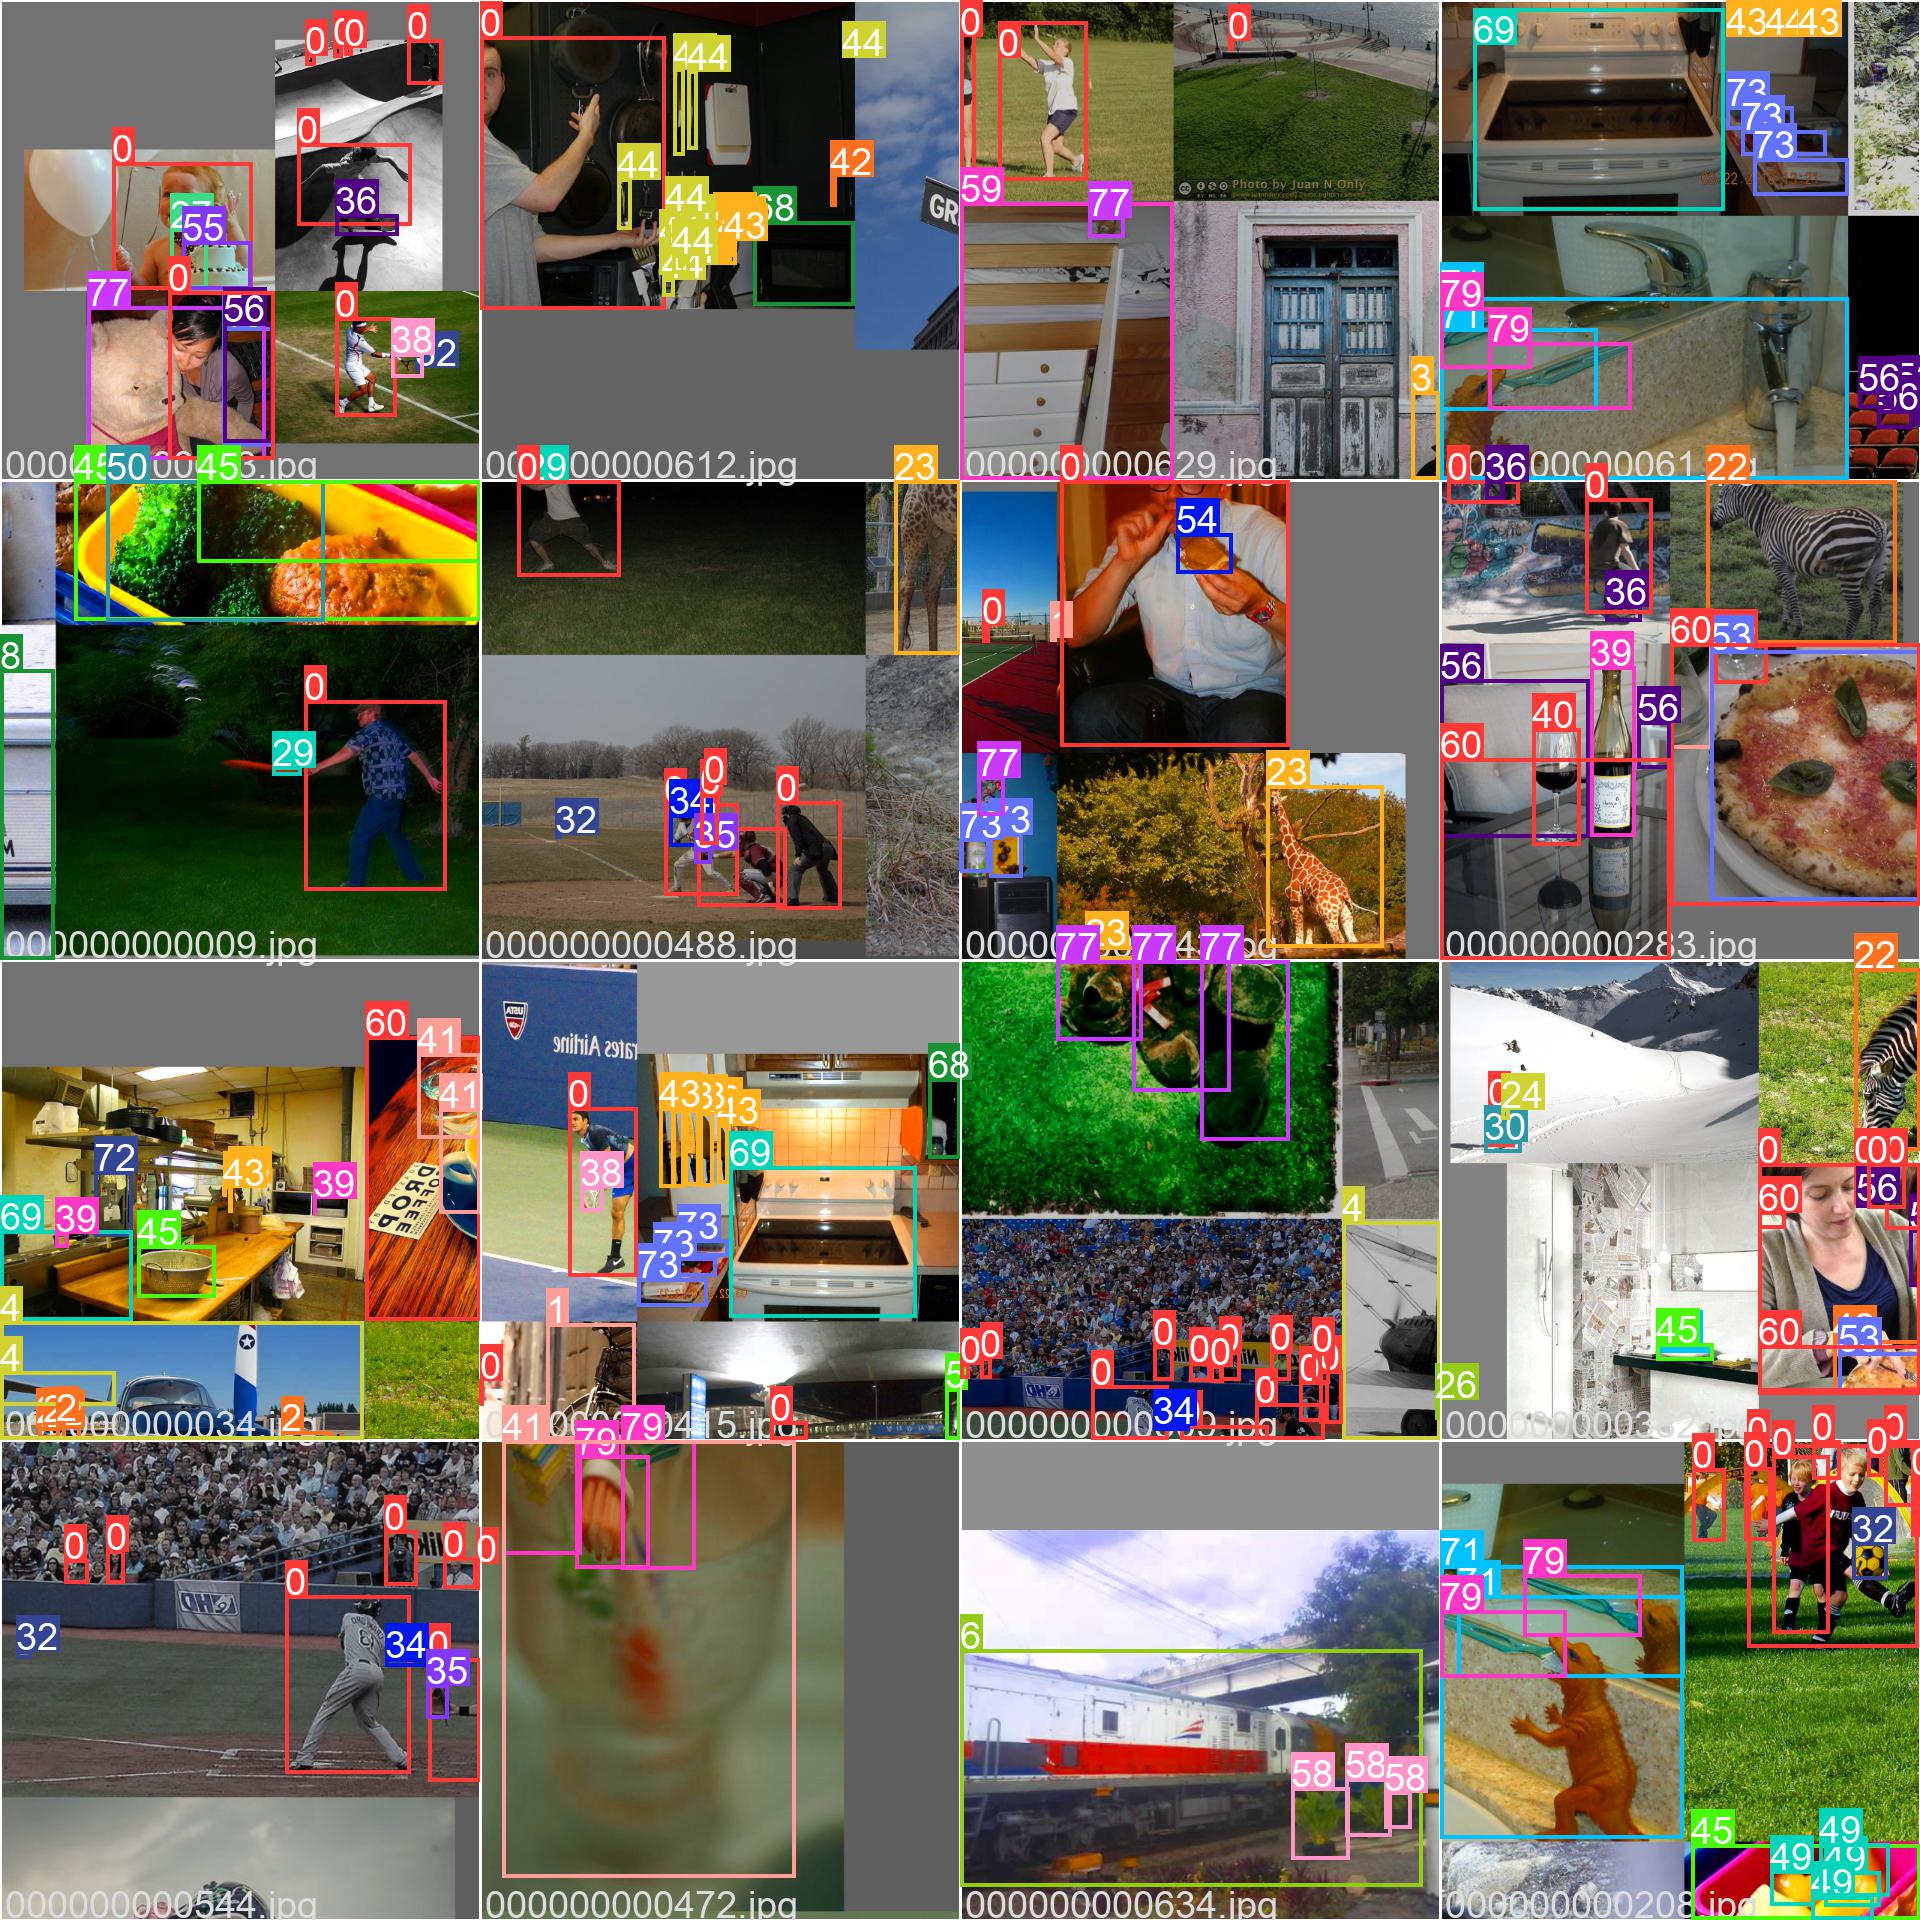
\includegraphics[width=0.8\textwidth]{figures/augmentation_ex.jpg}
    \end{center}
    \caption{Data Augmentation Example}
    \label{fig:data_augmentation}
\end{figure}


\subsubsection{Training Strategies}
YOLOv5 improves object detection accuracy by employing several training strategies.
The training strategies are multiscale training, auto-anchor, warm-up and cosine learning rate
scheduler, exponential moving average, mixed precision training and evolving hyperparameters.
These strategies improve precision without reducing frames per second by increasing training time.
YOLOv5 employs training at a scale of 0.5 to 1.5 times the input size.
Moreover, anchors are automatically generated and evolved to ensure that anchors are a suitable fit for
training data.
Next, warm-up and cosine learning rate configures the rate of learning rate.
Furthermore, exponential moving average maintains moving averages of variables by employing an exponential decay.
Finally, hyperparameters evolution is used to fine-tune model training.

% TODO: Maybe add Loss function
% TODO:Maybe add Eliminate Grid Sensitivity
% TODO: Maybe add Build Targets

\subsection{Simple, Online, Real-time Tracking (SORT)}
The SORT algorithm has three components, Estimation, Association and Tracking \cite{sort:2016}.
First, estimation is done by propagating the identity of a target into subsequent frames.
The state of a target is modelled using \ref{eq:estimate} where $u$ and $v$ is the coordinates of
the centre of a target.
In addition, $s$ and $r$ represent the area and aspect ratio of the bounding box of a target.

\begin{equation}
    x = [ u, v, s, r, \dot{u}, \dot{v}, \dot{s}] ^ T
    \label{eq:estimate}
\end{equation}

A Kalman filter is used to correct the new location of detections.
Next, the algorithm associates detections to targets.
The bounding box geometry of each target is estimated by predicting a new location in the current
frame.
A cost matrix is constructed using the intersection over union (IOU) distance between each detection
and all predicted bounding boxes from existing targets.
This assignment is solved using the Hungarian algorithm.
In addition, a minimum IOU is also set to reject probable targets with a low IOU.
Finally, tracking component handles the creation and deletion of objects.
A detection with an overlapping less than the minimum IOU is considered an untracked object.
The velocity component of this track is set to zero with the covariance of the velocity component at
a very large value to represent uncertainty.
A new track also requires to be detected consecutively for a set amount of frames before becoming a tracked
object.
Tracked objects are also terminated when they are not detected for a set amount of frames.

\clearpage

\chapter{Research Methodology}

\section{System Design}
An application is built written in C++ using the OpenCV library.
The source code is hosted on GitHub \cite{rvc-source:2022}.
In addition, the GitHub repository includes build instructions and the requirements to run and build the
application.
An overview of this application is shown in Fig. \ref{fig:systemflow}.

\begin{figure}[htbp]
    \begin{center}
        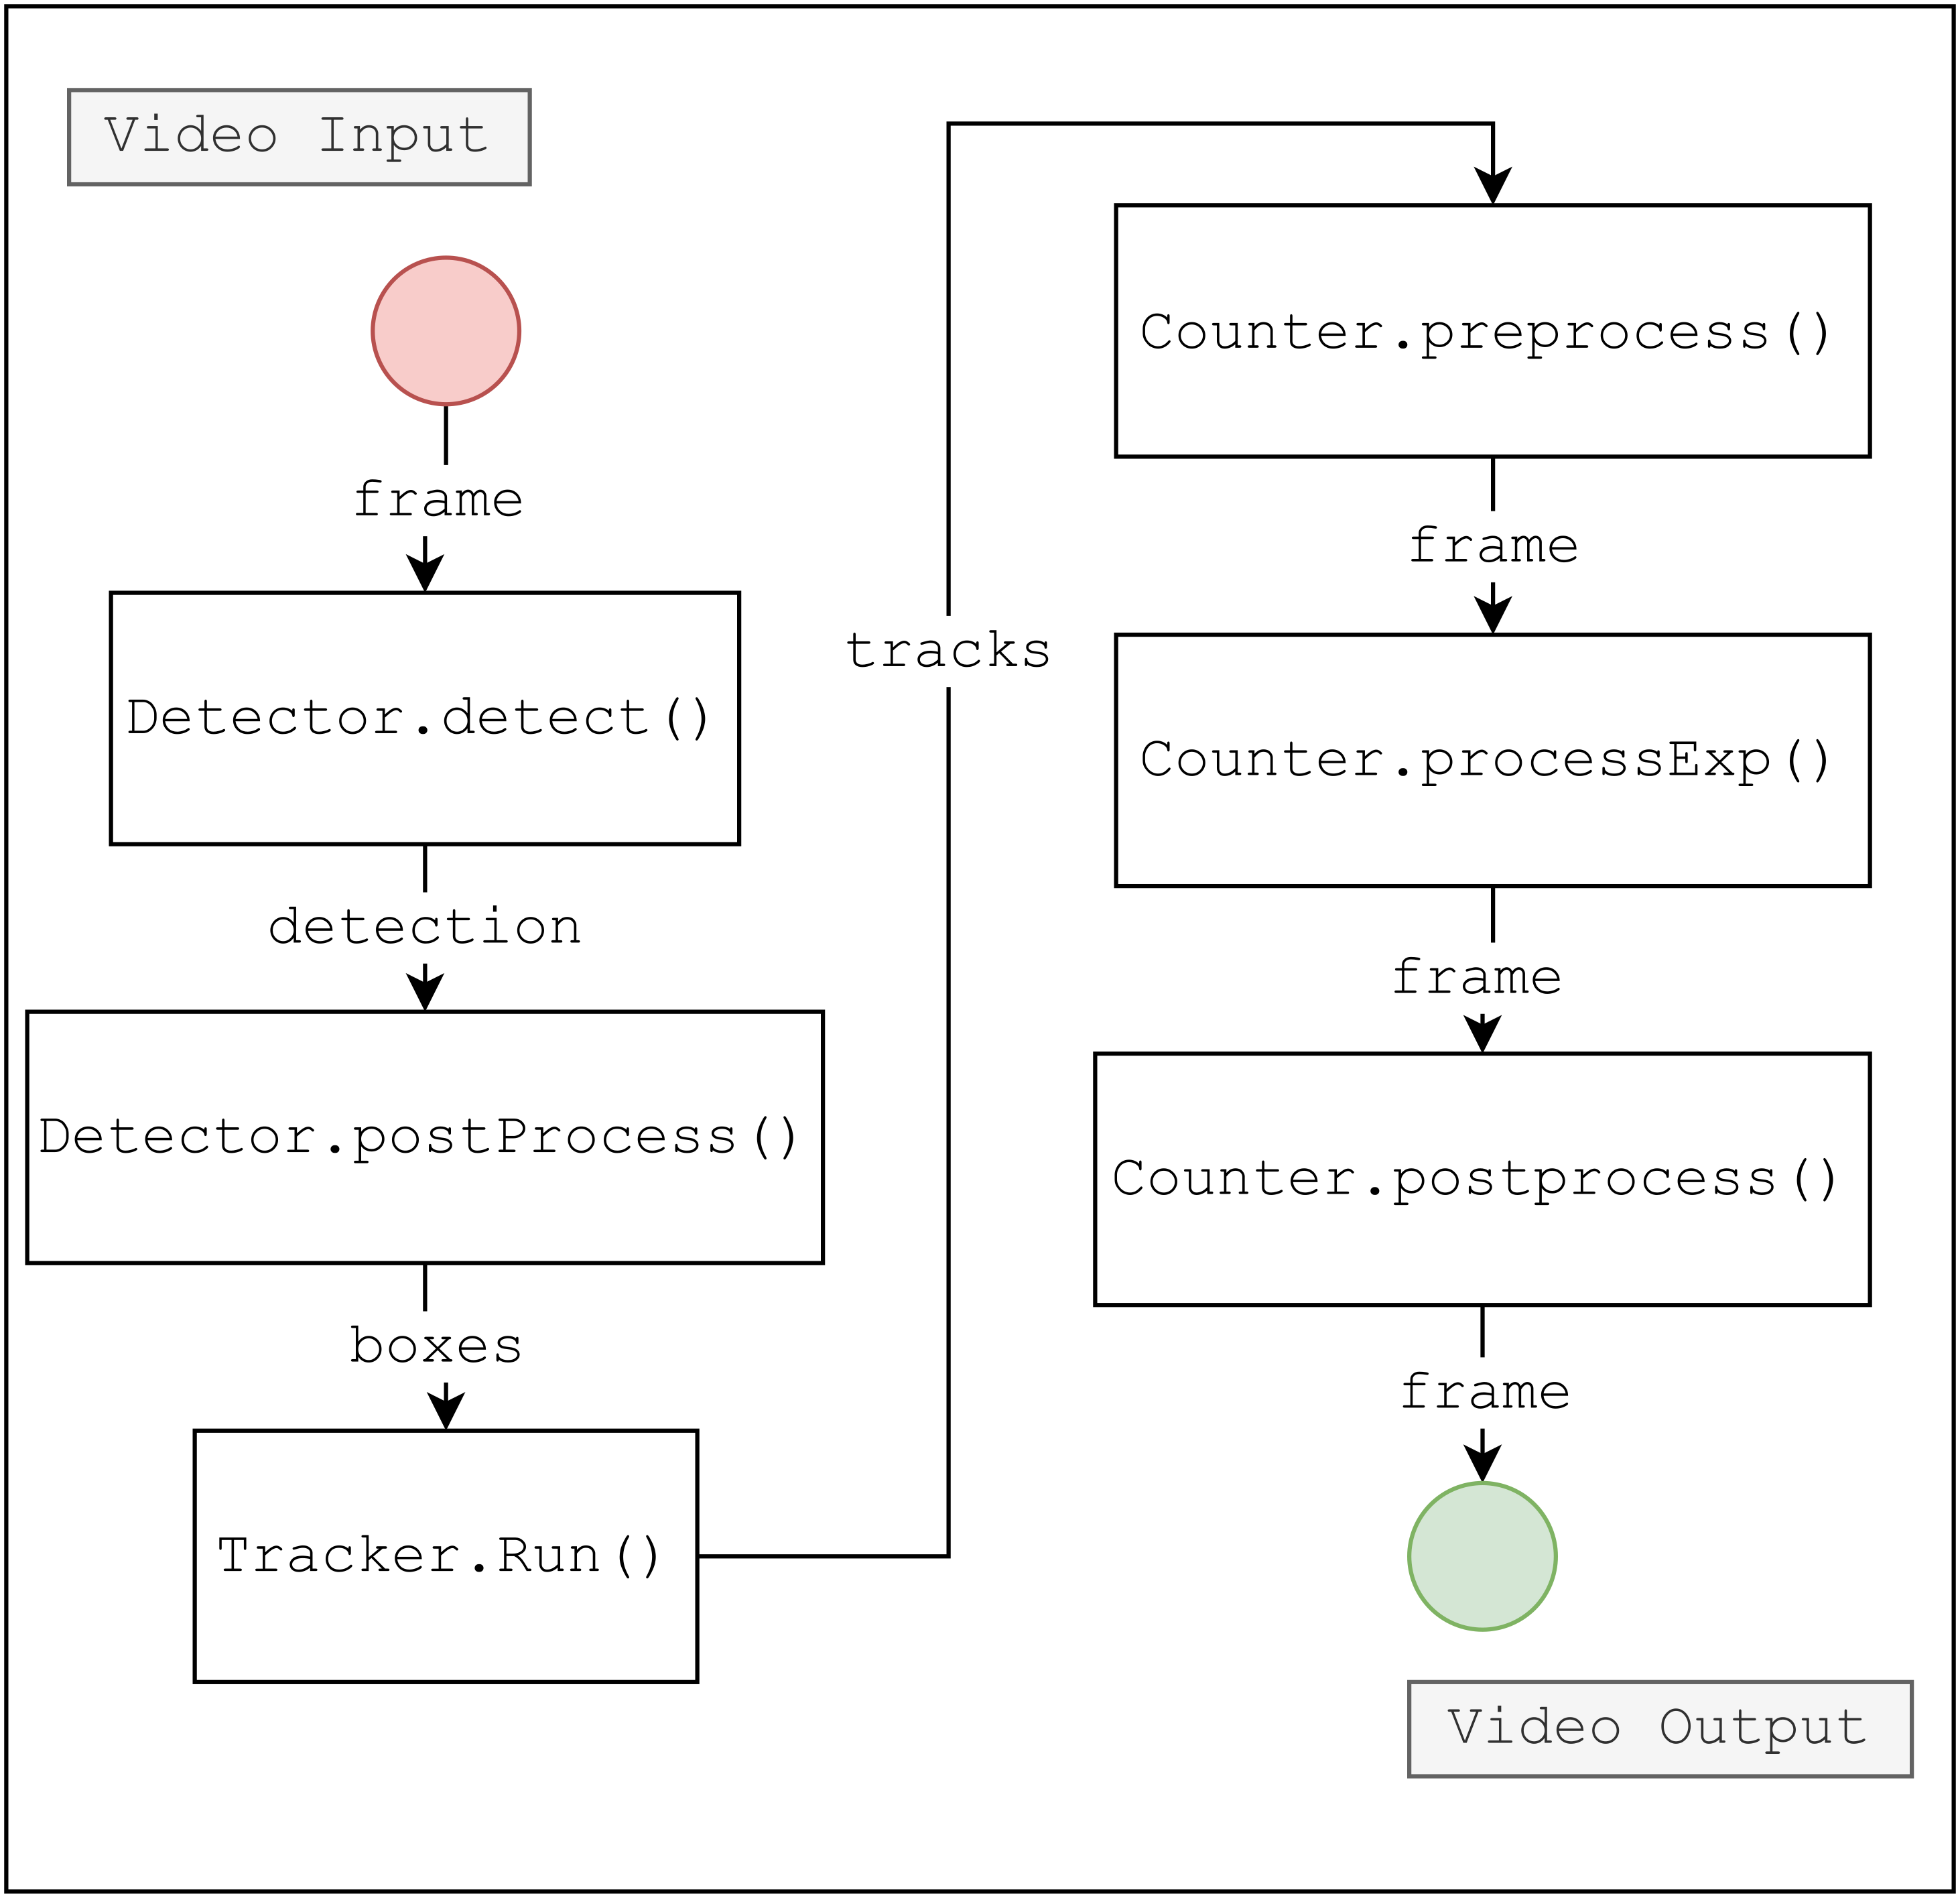
\includegraphics[width=0.65\textwidth]{figures/systemflow.png}
    \end{center}
    \caption{Overview of Application Flow}
    \label{fig:systemflow}
\end{figure}

\begin{figure}[htbp]
    \begin{subfigure}[htbp]{0.5\textwidth}
        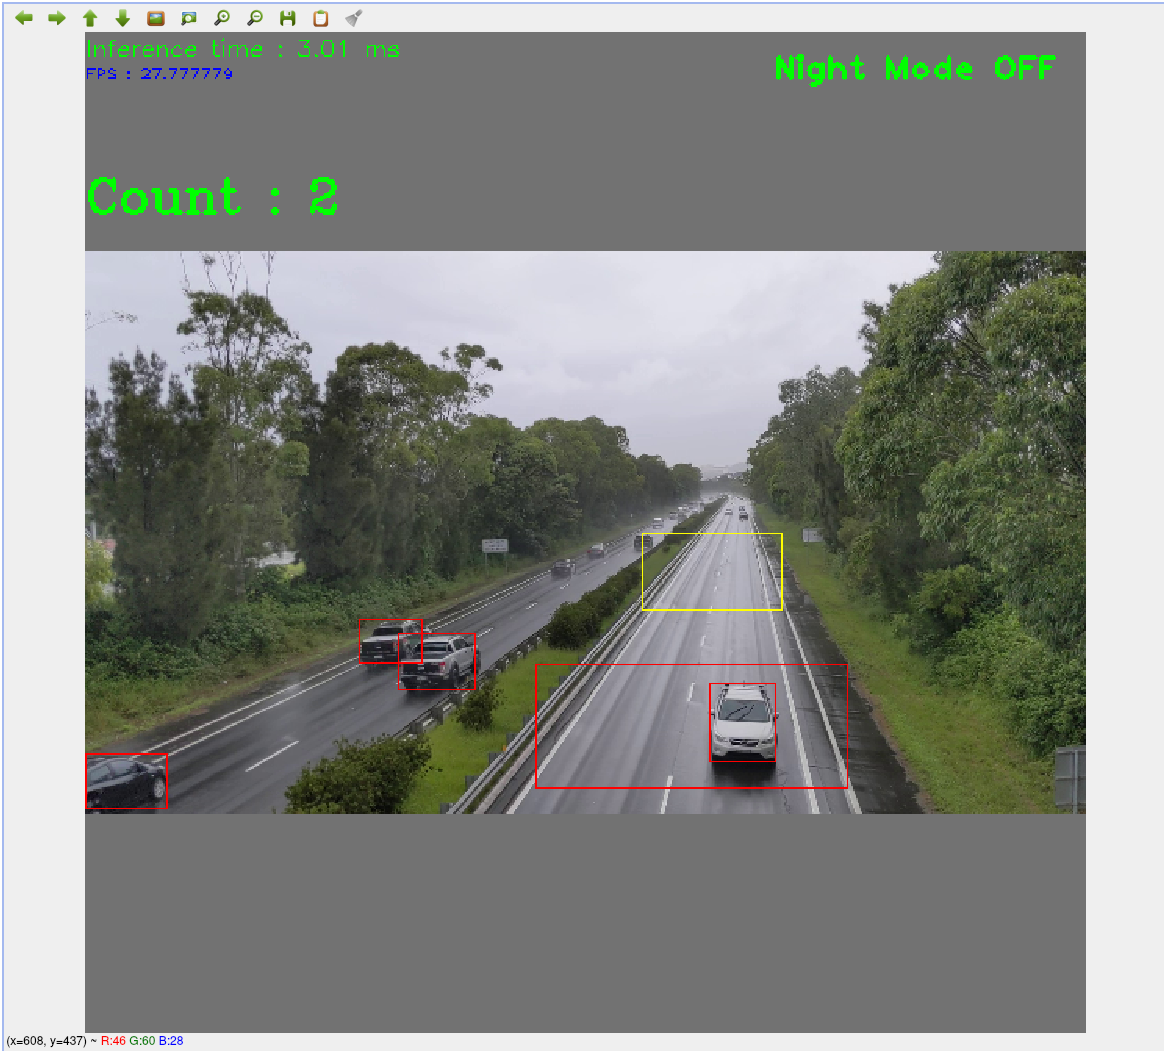
\includegraphics[width=0.95\textwidth]{figures/daytime-detection.png}
    \caption{Daytime Counting}
    \label{fig:daytime-detection}
    \end{subfigure}
    \begin{subfigure}[htbp]{0.5\textwidth}
        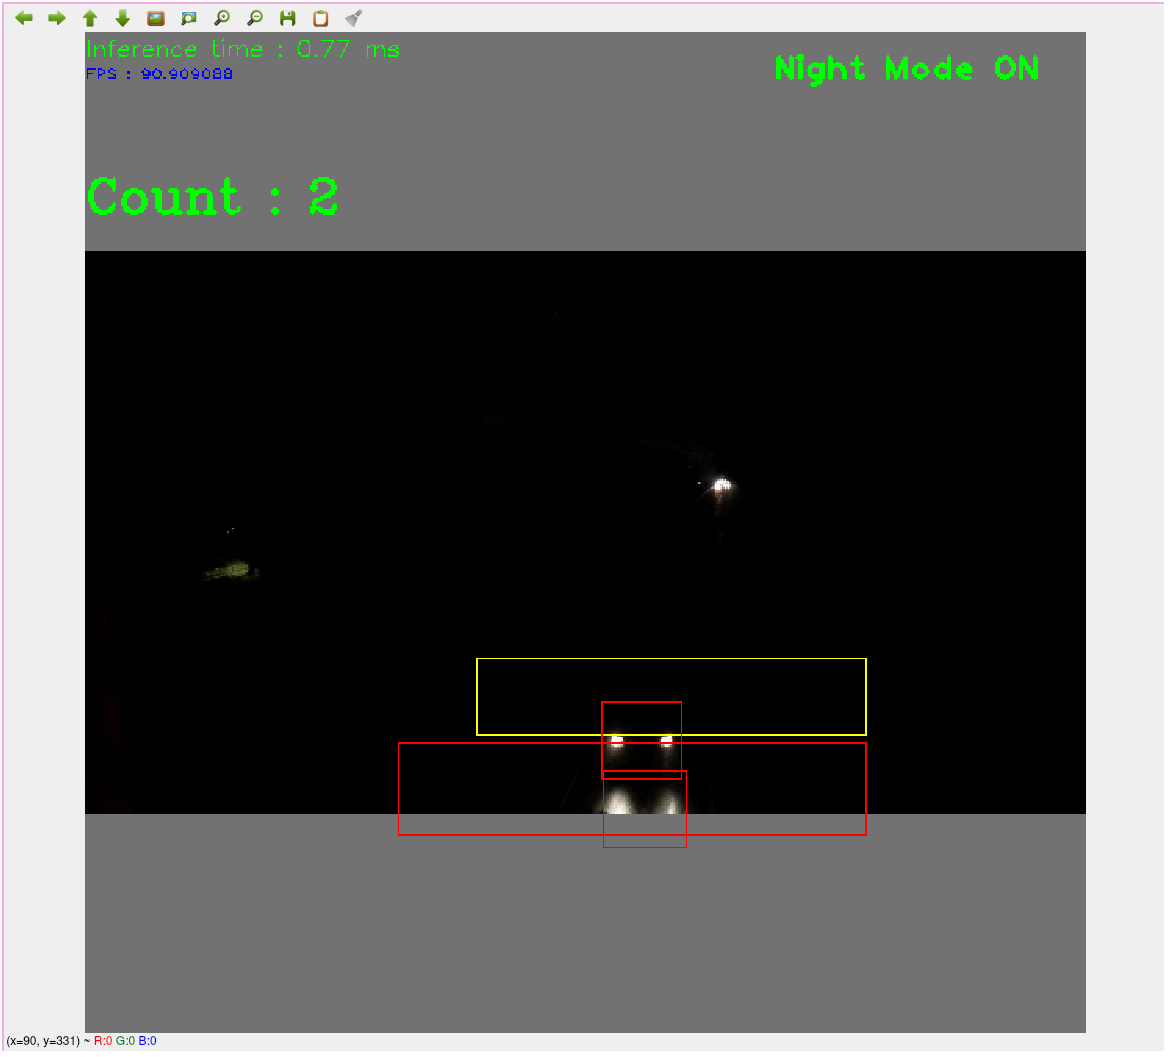
\includegraphics[width=0.95\textwidth]{figures/nightime-detection.png}
    \caption{Nighttime Counting}
    \label{fig:nighttime-detection}
    \end{subfigure}
    \caption{Detection, Tracking and Counting}
    \label{fig:detection-tracking-counting}
\end{figure}


\subsection{Detection}
The application uses the OpenCV Deep Neural Networks module and YOLOv5 for daytime object detection.
The universal sample in \cite{opencvyolosample:2022} is heavily modified to be more modular and
accommodate the YOLOv5 network.
On the other hand, nighttime detection is uses image thresholding and headlight matching.
The application automatically switches to nighttime detection when the two \mintinline{bash}{night_roi_x}
areas are completely black.
Daytime detection and nighttime detection is shown in Fig. \ref{fig:daytime-detection} and Fig.
\ref{fig:nighttime-detection} respectively.
First, a detector class is initialised with the configuration from the command line.
Next, video frames from the camera is passed into the detect function.
The appropriate detection function is called for daytime and nighttime detection.
The daytime object detector first resizes the input to match the requirements for the neural network.
The convolutional neural network is read using the ONNX extension type.
The output from the CNN is also passed into the NMSBoxes function from OpenCV which selects the most
accurate boxes given a set of overlapping bounding boxes.
This is done using Non-maximum Suppression (NMS).
The output from the NMSBoxes function is then passed to the tracker.

The nighttime object detector also resizes the input to match with the daytime detection outputs.
First, image processing is used to reduce the noise in the input.
A Gaussian blur with a kernel size of 3 is used to reduce input noise.
Next, pixels are set to 0 or 1 using the OpenCV threshold function.
The resulting input is then eroded and dilated to further focus on the bright blobs in the input.
All bright blobs are considered and the size, height and location of the blob is used for
headlight matching.
In this case, headlight matching has several rules.
First, the area of pairs should be within $\pm100$ pixels squared.
Next, the height difference of headlight pairs should be within $\pm 10$ pixels.
Finally, the width difference of headlight pairs should be greater than $20$ pixels and smaller than $80$
pixels.
Matched contours are provided a bounding box which is passed to the tracker.


\subsection{Tracking}
The tracker uses the Simple, Online, Real-time Tracking algorithm.
This is handled using a tracker and track class.
The track class represents a tracked object.
The tracker class handles all operations for the SORT algorithm.
The \mintinline{c++}{Tracker::Run()} function is the main component of this class.
It accepts detections as arguments.
First, this function first estimates the internal next states of tracked objects.
Next, the function then associates detections to tracks using a generated cost matrix based on the number
of detections and tracks.
Hungarian matching is used to associate detections to tracks.
The IOU threshold is used to filter matches with a low IOU.
If detections have yet to be associated to a track, it will create a new track item.
When tracks have not been detected for a set amount of iterations, it will be erased from the list
of tracks.
Finally, this output is passed to the counter.


\subsection{Counting}
The application uses a simple Counter class which accepts track objects as inputs.
This counter class establishes two regions of interest in the input frame.
Next, the counter processes each track to find if each tracks intersect with the predefined regions
of interest.
If the track has not previously intersected with the region of interest, it will be added to a vector.
This vector contains the ID of tracked object and the count which it has been missing.
In this case, missing tracks are removed after 200 iterations.
If the track has intersected with both regions of interest, the application will increment the
counter and the ID of tracked object removed from both intersection vectors.
Finally, the object count is put onto the screen.
This counter class can count objects regardless of sequence of objects passing through.
An overview of this counter class is presented in Fig. \ref{fig:counterflow}.

\begin{figure}[htbp]
    \begin{center}
        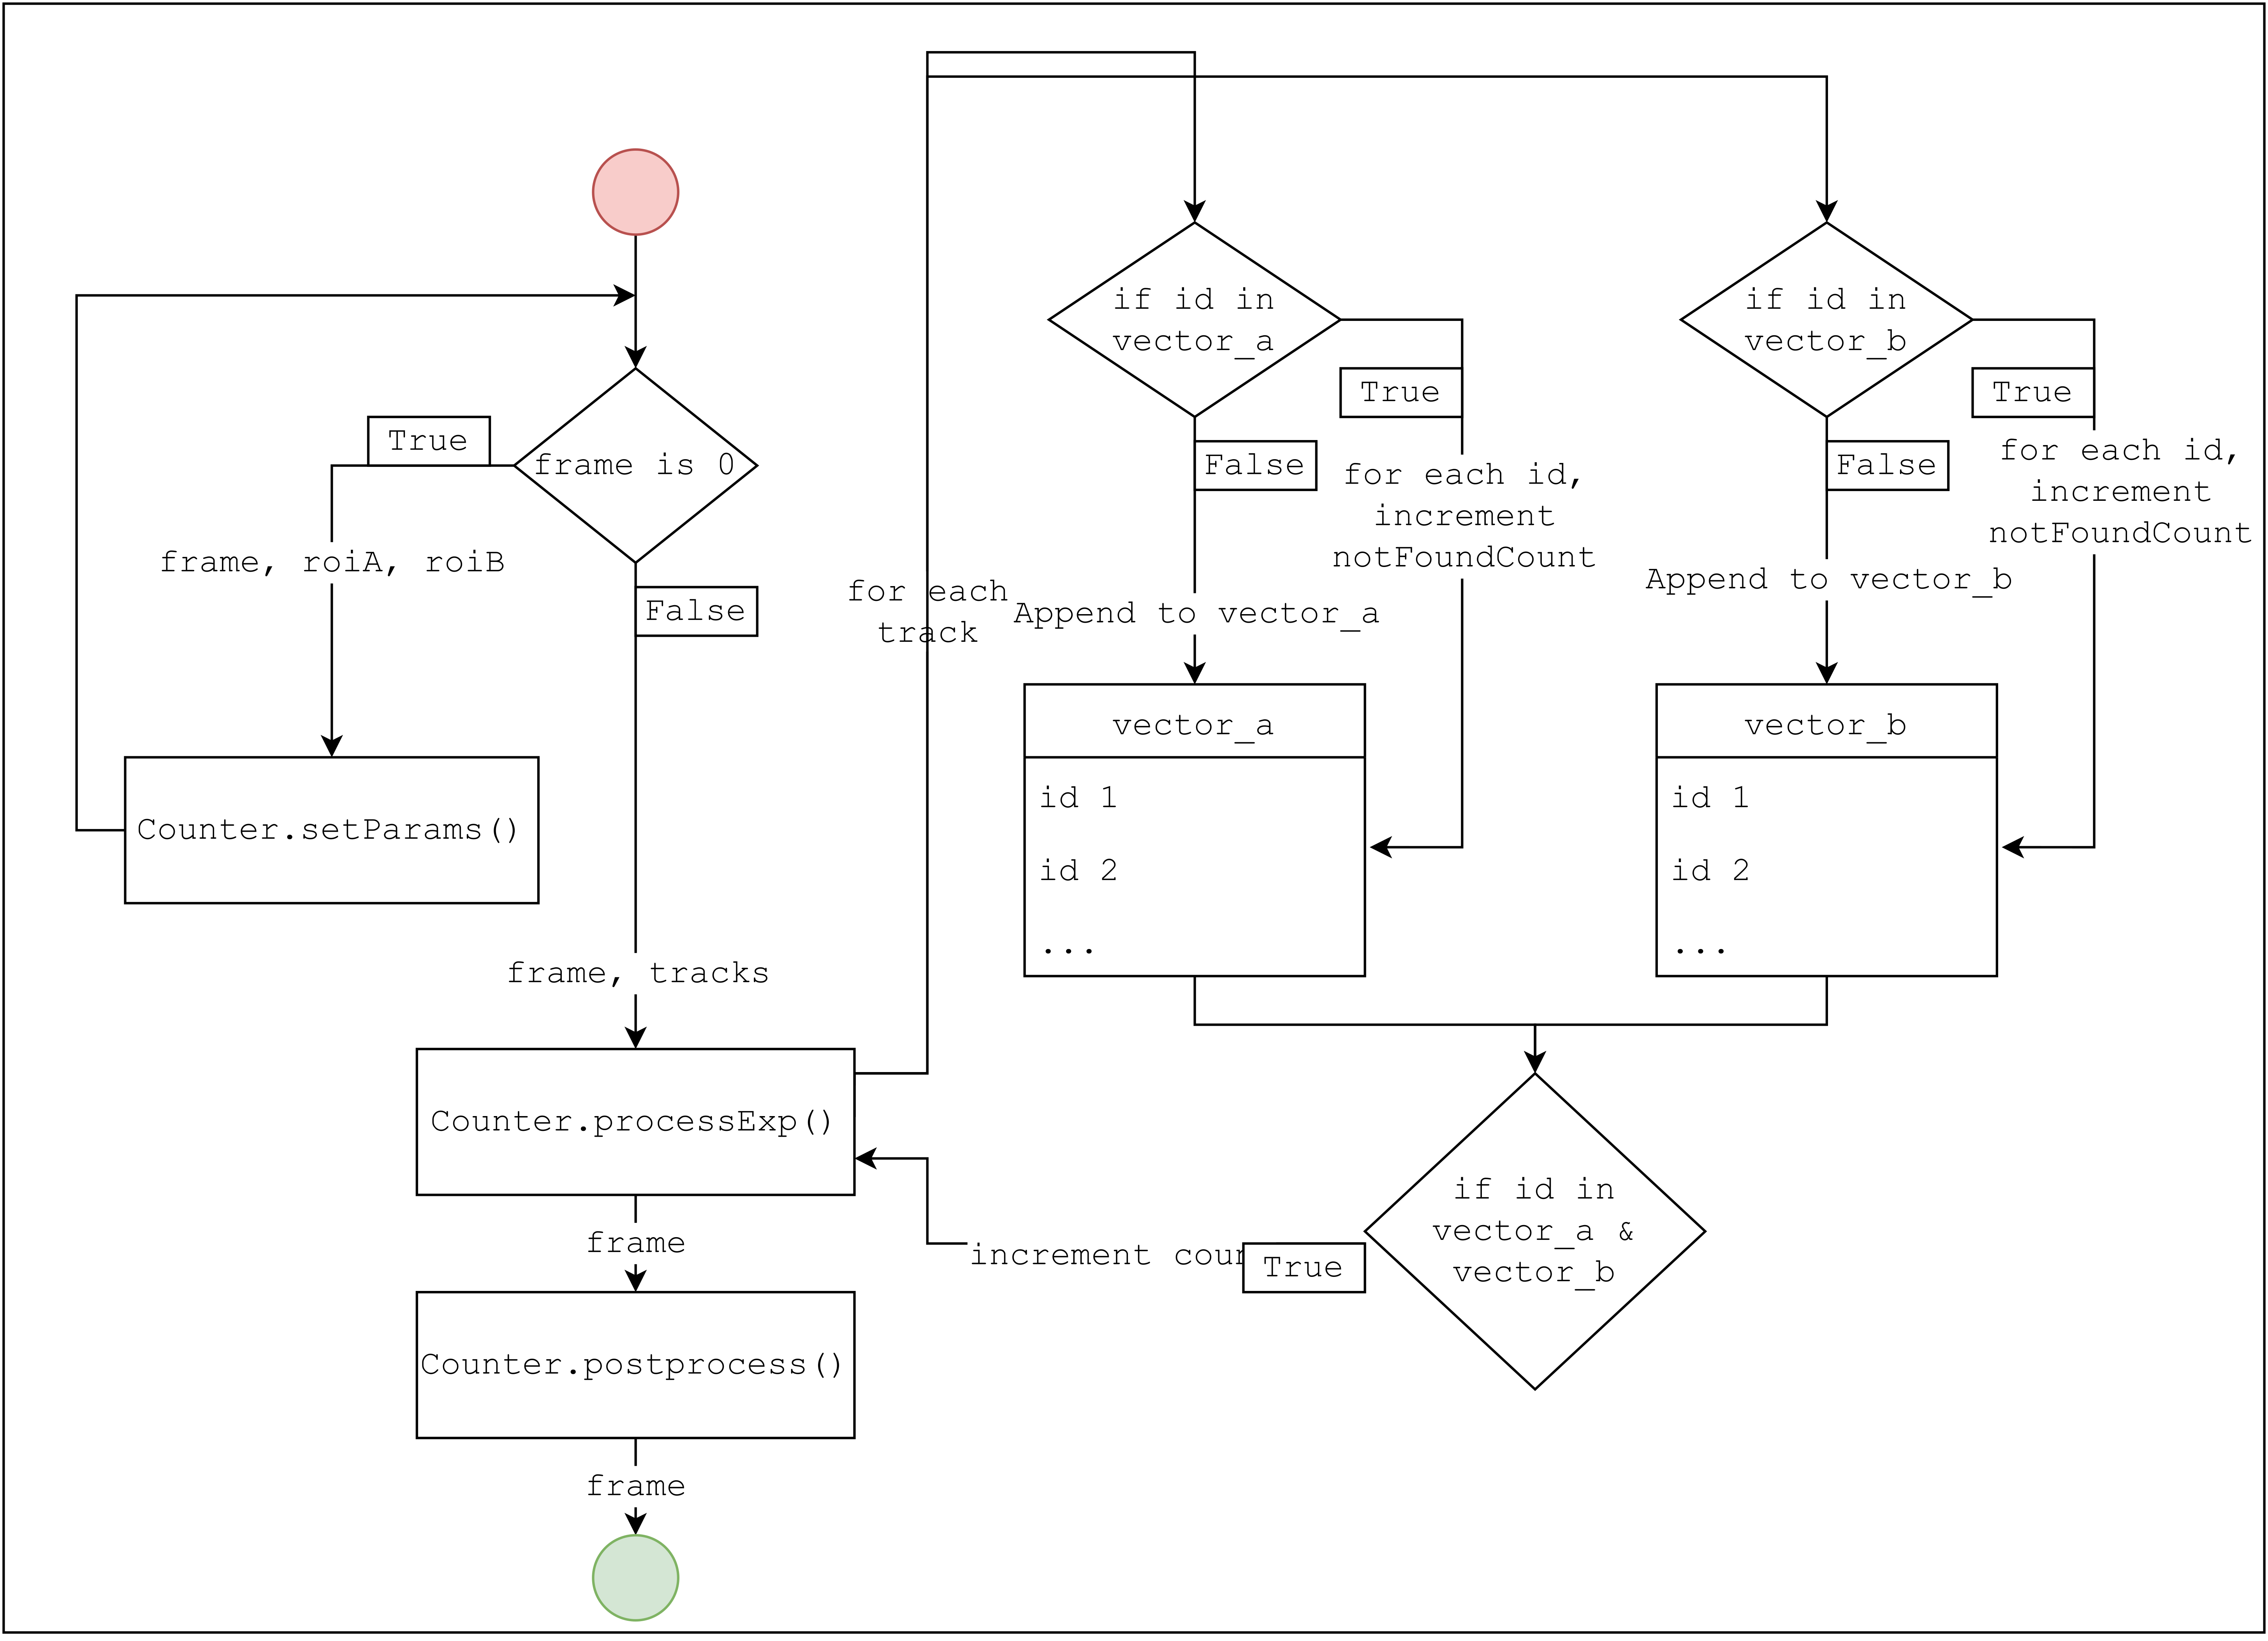
\includegraphics[width=0.9\textwidth,height=8cm]{figures/counterflow.png}
    \end{center}
    \caption{Overview of Counter Class}
    \label{fig:counterflow}
\end{figure}


\subsection{User Interface}
A terminal user interface (TUI) shown in Fig. \ref{fig:rvc-tui} is created using Python and PyTermGui \cite{pytermgui:2022}.
This TUI enables a user to interface with the application without using the command line.
In addition, Listing \ref{lst:cla} shows that the project can be started in the terminal.
The parameters of the application can be set using the input on the TUI.
\mintinline{bash}{ROI x} sets the region of interest for vehicle counting.
Next, \mintinline{bash}{Night Mode ROI x} sets the region of interest which triggers nighttime object
detection.
Moreover, the \mintinline{bash}{Preview Toggle} determines if the application should start with a
preview before starting the counter.
The object detection model can be selected using the \mintinline{bash}{Select Deep Learning Model}
button.
Next, the \mintinline{bash}{Set} button sets the parameters to run the application.
The preview screen can be switched to the counting screen by pressing \mintinline{bash}{s}.
The counting program can be stopped by pressing \mintinline{bash}{ESC}.
Finally, the \mintinline{bash}{Start} button starts the real-time vehicle counting application.

\begin{figure}[htbp]
    \begin{center}
        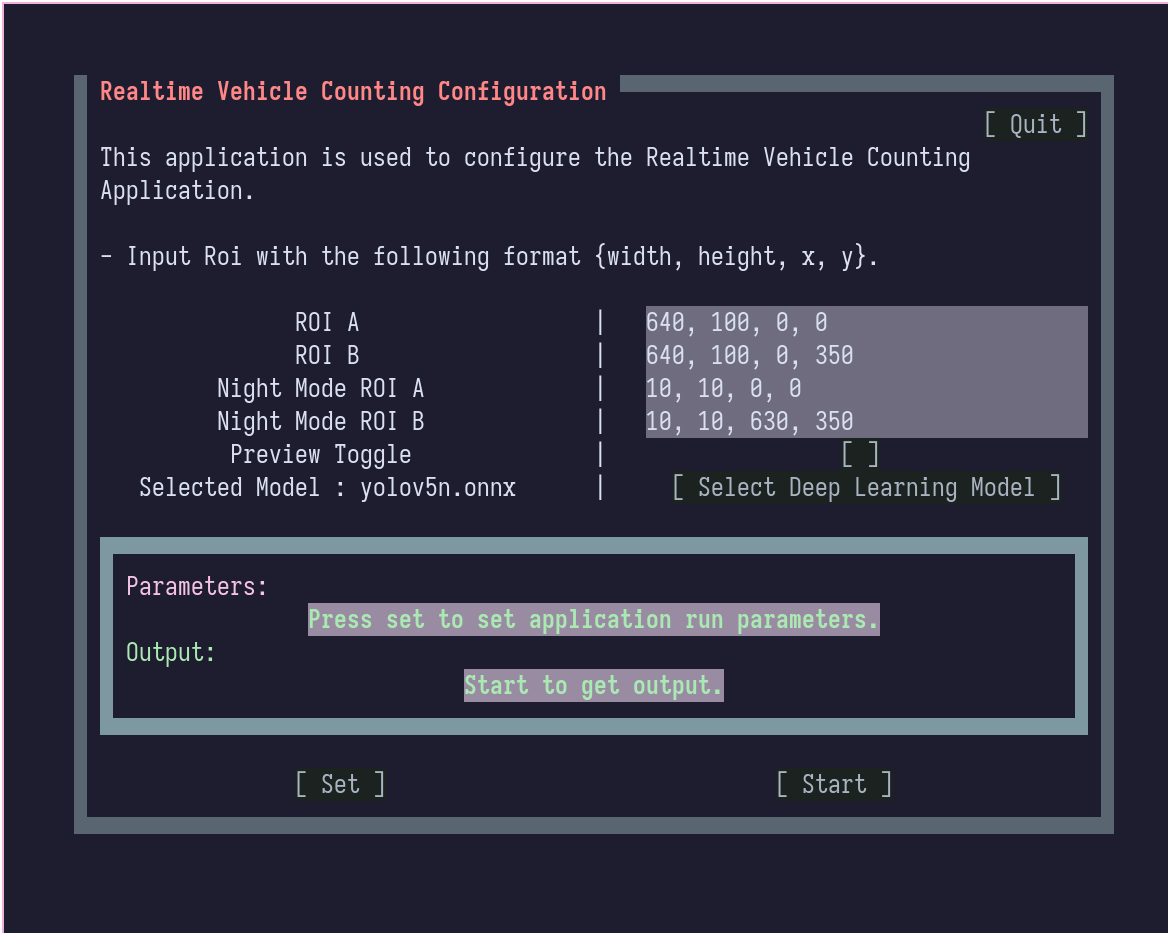
\includegraphics[width=0.8\textwidth]{figures/rvc-tui.png}
    \end{center}
    \caption{User Interface of Application}
    \label{fig:rvc-tui}
\end{figure}



\begin{listing}[htbp]
\definecolor{bg}{rgb}{0.95,0.95,0.95}
\begin{minted}[
frame=lines,
framesep=2mm,
baselinestretch=1.0,
fontsize=\footnotesize,
bgcolor=bg,
linenos,
]{bash}
# test_video
./build/realtime-counting \
    --model_path="./dnn_files/yolov5n.onnx" \
    --class_path="./dnn_files/coco_c.names" \
    --model_size=640 \
    --roi_A=640,100,0,0 \
    --roi_B=640,100,0,350 \
    --actual_count=239

# rain_high_angle
./build/realtime-counting \
    --model_path="./dnn_files/yolov5n.onnx" \
    --class_path="./dnn_files/coco_c.names" \
    --model_size=640 \
    --roi_A=90,50,356,320 \
    --roi_B=200,80,288,404 \
    --actual_count=368

# night_high_angle
./build/realtime-counting \
    --model_path="./dnn_files/yolov5n.onnx" \
    --class_path="./dnn_files/coco_c.names" \
    --model_size=640 \
    --roi_A=250,50,200,400 \
    --roi_B=300,60,190,454 \
    --night_mode=1 \
    --actual_count=101

# night_high_angle_low_exposure
./build/realtime-counting \
    --model_path="./dnn_files/yolov5n.onnx" \
    --class_path="./dnn_files/coco_c.names" \
    --model_size=640 \
    --roi_A=250,50,200,400 \
    --roi_B=300,60,190,454 \
    --night_mode=1 \
    --actual_count=105 \

\end{minted}
\caption{Running with the Command Line}
\label{lst:clrun}
\end{listing}

\clearpage

\section{Experiment Methodology}
The experiment was conducted in two locations both of which are above a highway.
The highways are Princes Motorway and Memorial Drive respectively.
Video footage of both locations are recorded using the main camera of a Pixel 4 at 1080p 30FPS.
The Google Pixel 4 was secured using a tripod and put near the railing of the bridge for stability.
This is shown in Fig. \ref{fig:experiment_setup}.
The location and footage location for each video are shown in Table \ref{tab:expvidparam}.

\begin{figure}[htbp]
    \centering
    \begin{subfigure}[htbp]{0.48\textwidth}
        \begin{center}
            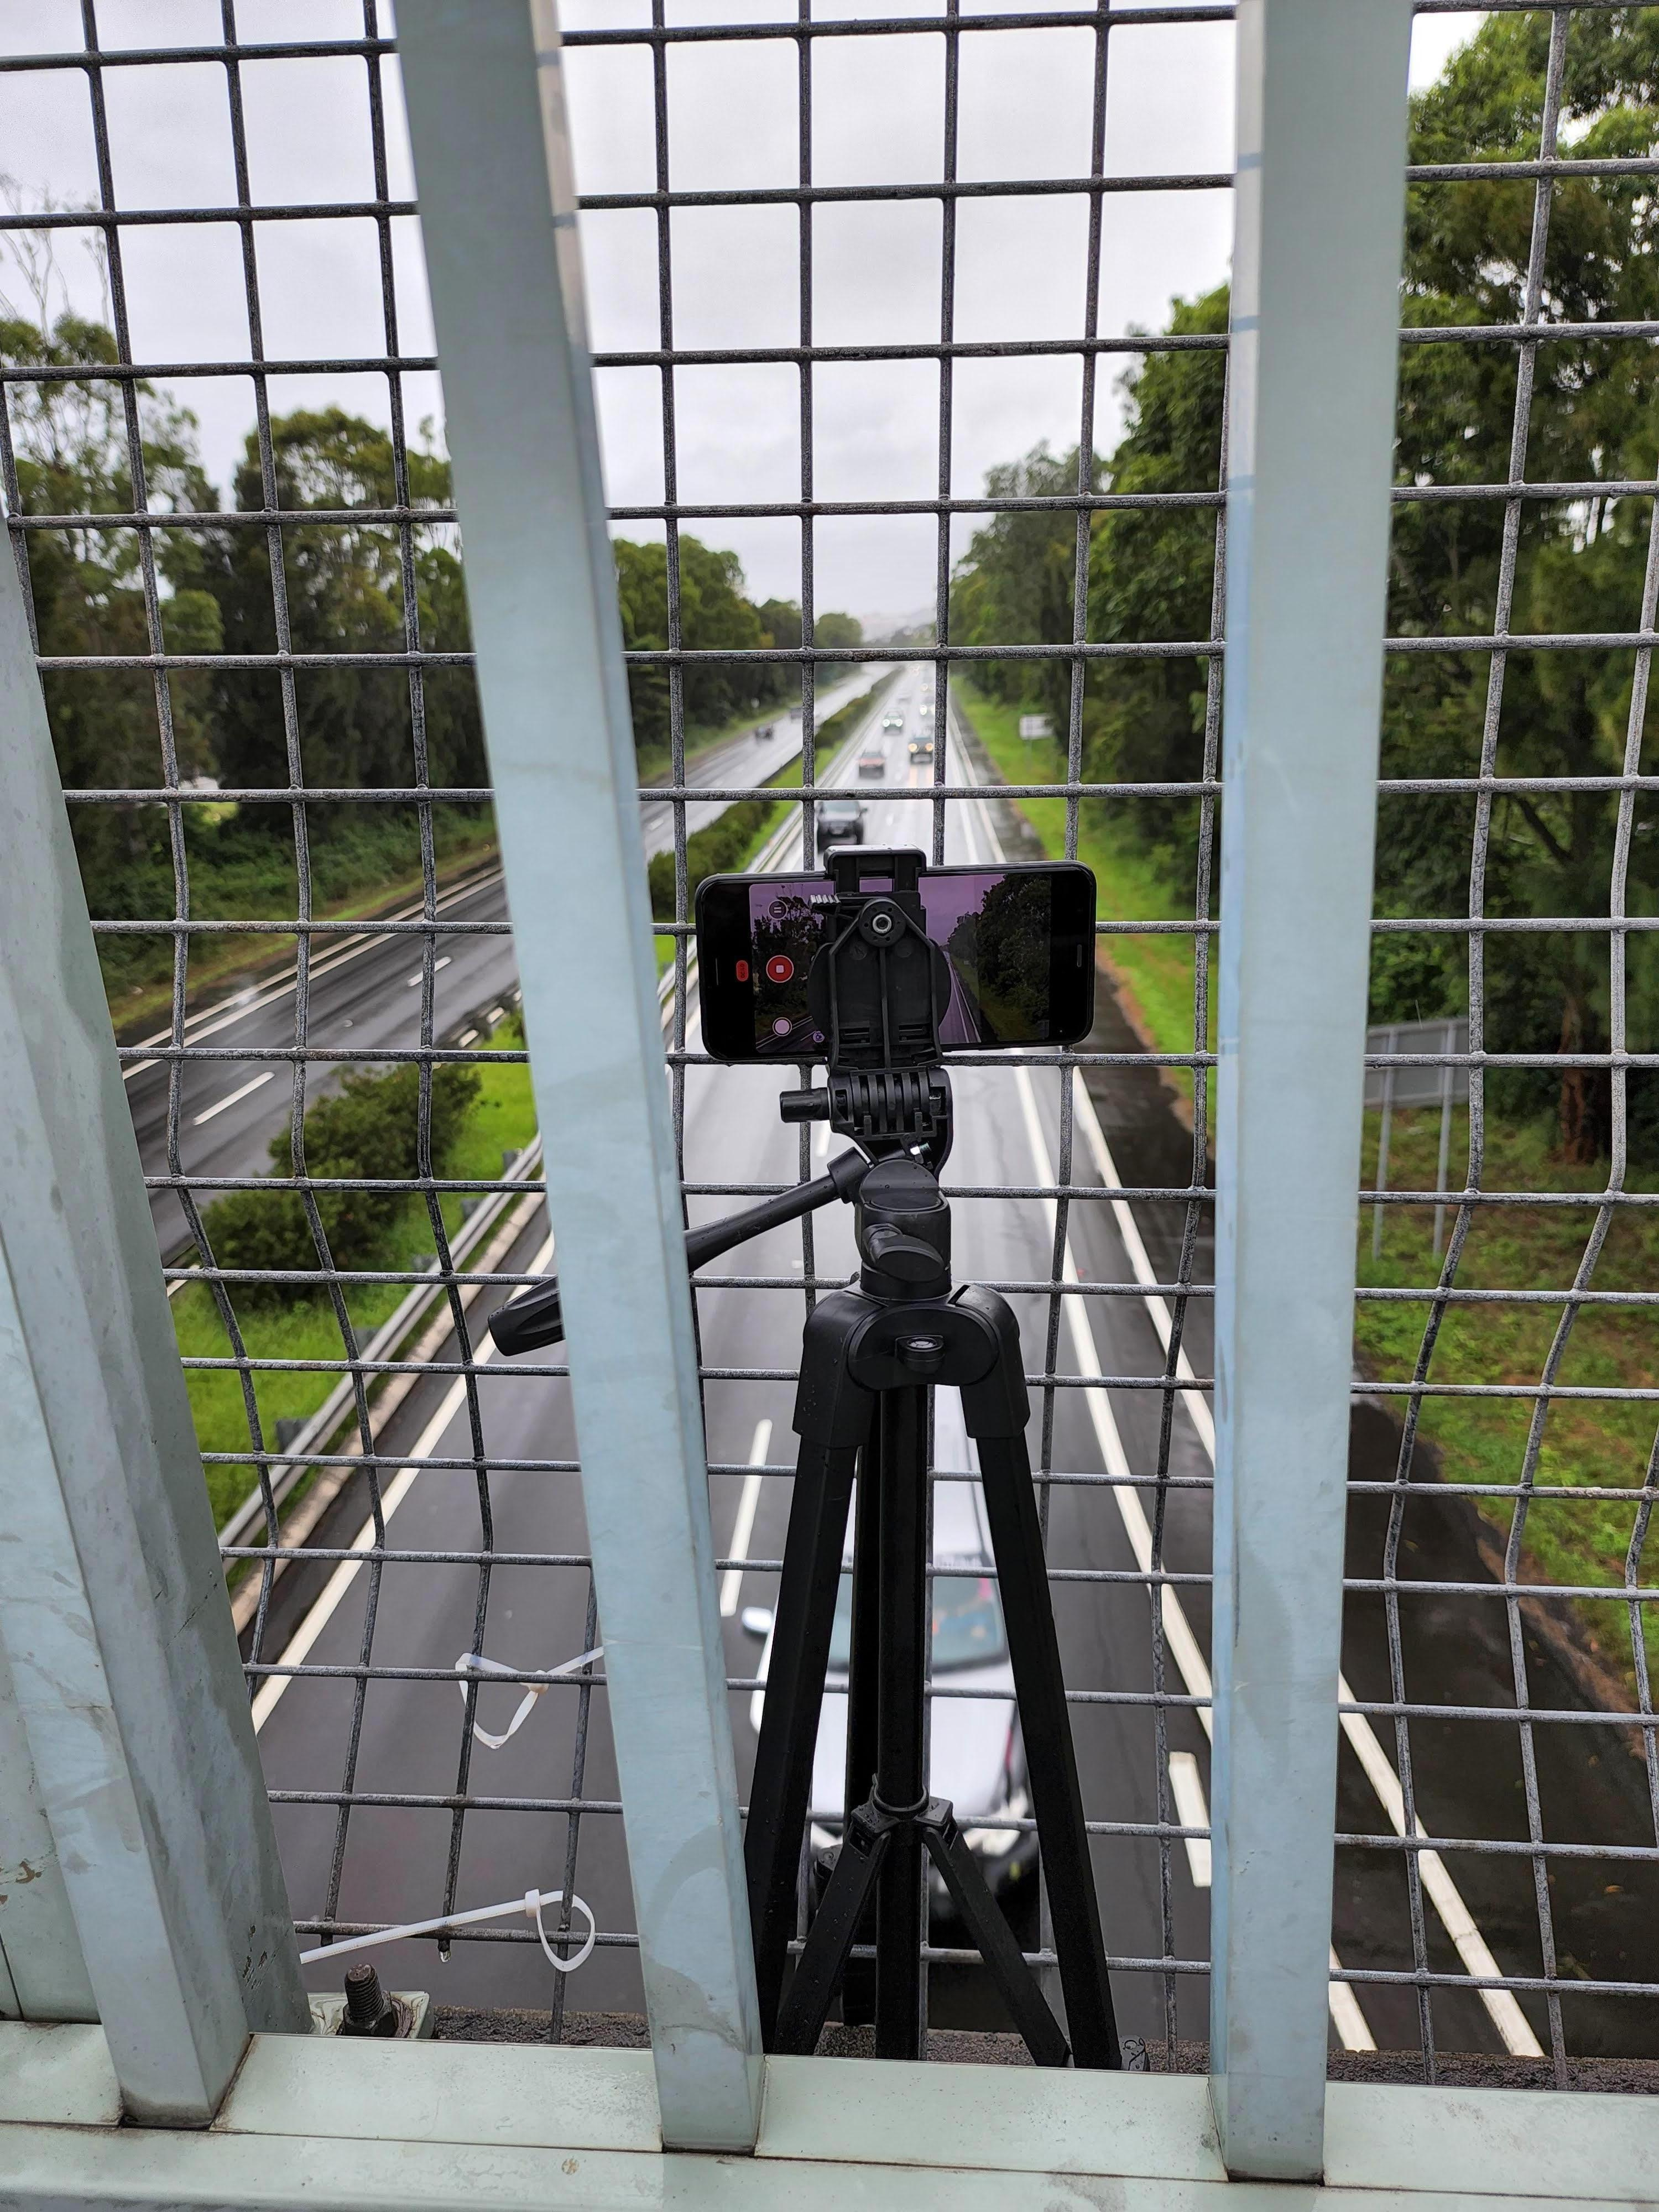
\includegraphics[width=0.9\textwidth,height=8cm]{figures/experiment_setup.jpg}
        \end{center}
        \caption{Daytime Setup}
        \label{fig:daytime_exp}
    \end{subfigure}
    \begin{subfigure}[htbp]{0.48\textwidth}
        \begin{center}
            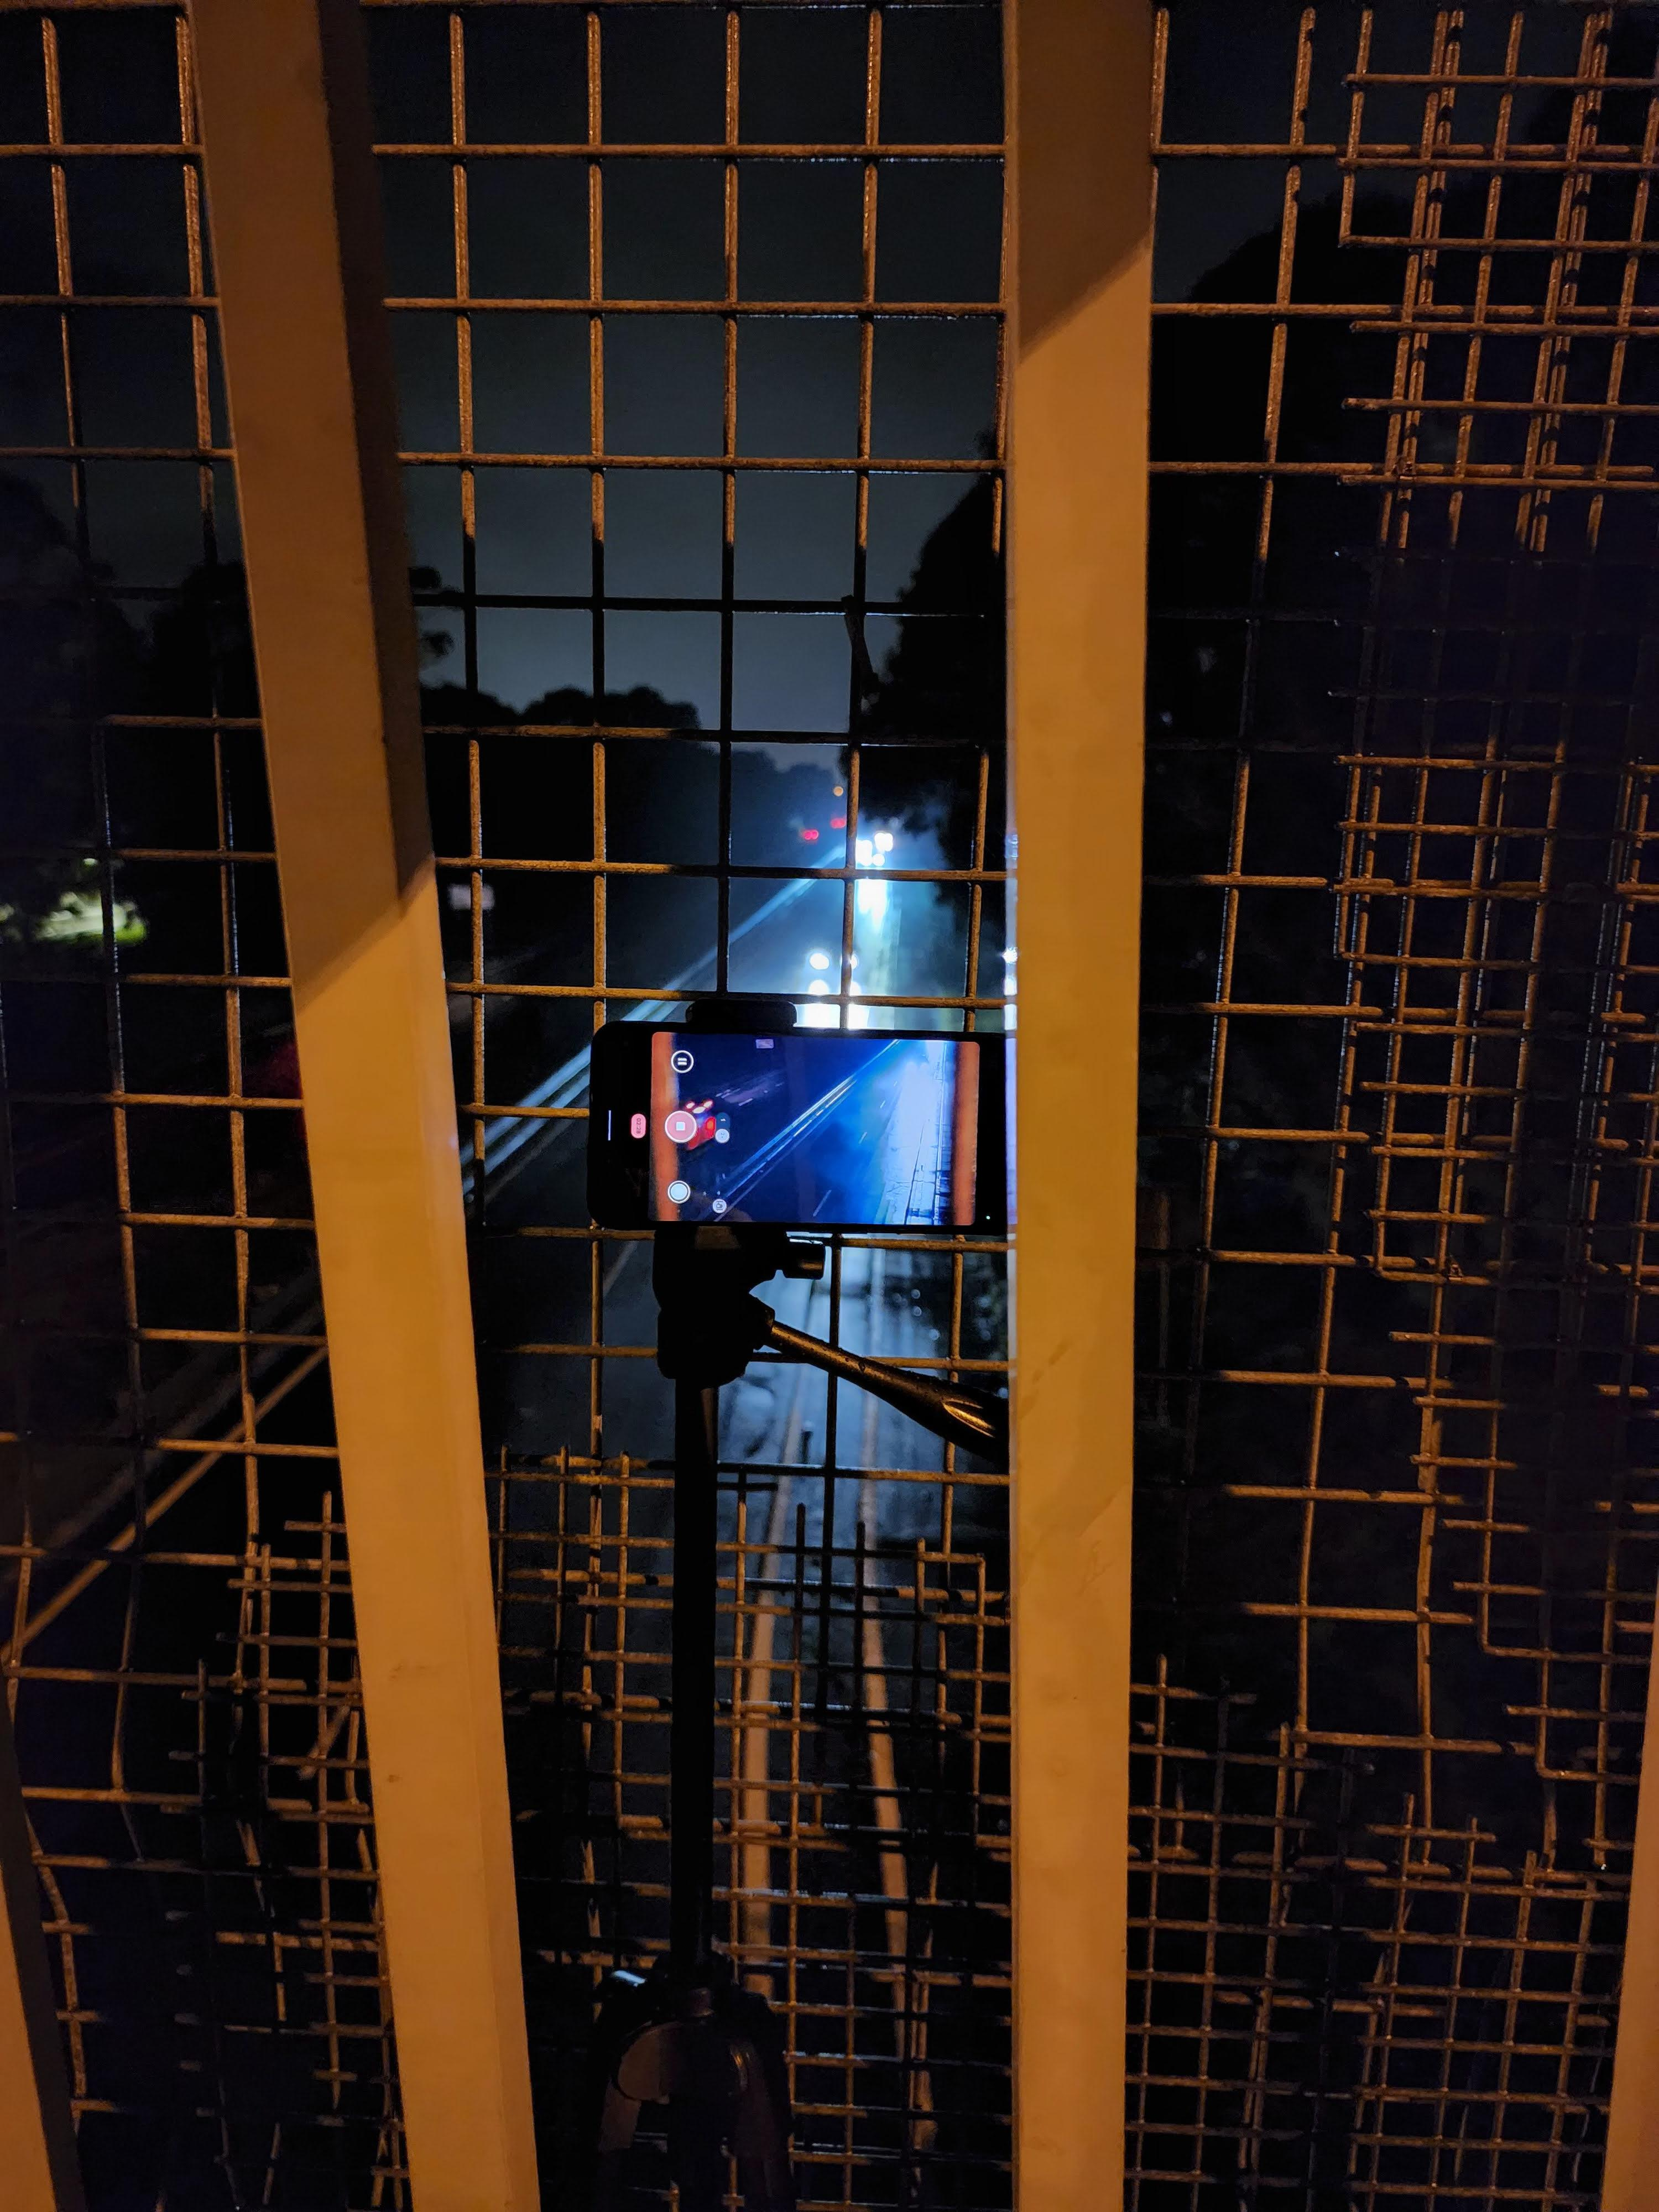
\includegraphics[width=0.9\textwidth,height=8cm]{figures/night_time_setup.jpg}
        \end{center}
        \caption{Nighttime Setup}
        \label{fig:nighttime_exp}
    \end{subfigure}
    \caption{Experiment Setup: Footage Collection using a Pixel 4 and Tripod}
    \label{fig:experiment_setup}
\end{figure}


\begin{table}[htbp]
    \centering
    \begin{adjustbox}{width=1\textwidth}
    \begin{tabular}{|l|l|l|l|}
    \hline
    \textbf{Video Name} & \textbf{Duration} & \textbf{Location Coordinates} & \textbf{Target Highway} \\ \hline
    \textbf{test\_video} & 10 mins 58 secs & -34.410872, 150.882943 & Princes Motorway \\ \hline
    \textbf{rain\_high\_angle} & 10 mins 53 secs & -34.394881, 150.896032 & Memorial Drive \\ \hline
    \textbf{night\_high\_angle} & 12 mins 16 secs & -34.394881, 150.896031 & Memorial Drive \\ \hline
    \textbf{night\_high\_angle\_low\_exposure} & 11 mins 11 secs & -34.394881, 150.896032 & Memorial Drive \\ \hline
    \end{tabular}
\end{adjustbox}
\caption{Video Parameters}
\label{tab:expvidparam}
\end{table}

The experiment uses the Open Broadcaster Software (OBS) to simulate accessing the camera on-site.
This is shown in Fig. \ref{fig:exp_sim_obs}.
OBS can generate a virtual camera which can be accessed using OpenCV.
This is because the \mintinline{c++}{VideoCapture.read()} function does not read video frames according to time.
As presented in Listing \ref{lst:experiment}, this program will wait 1 ms at best effort before reading
each frame.
However, the program will be able to finish reading the video faster than actual time.

\begin{figure}
    \begin{center}
        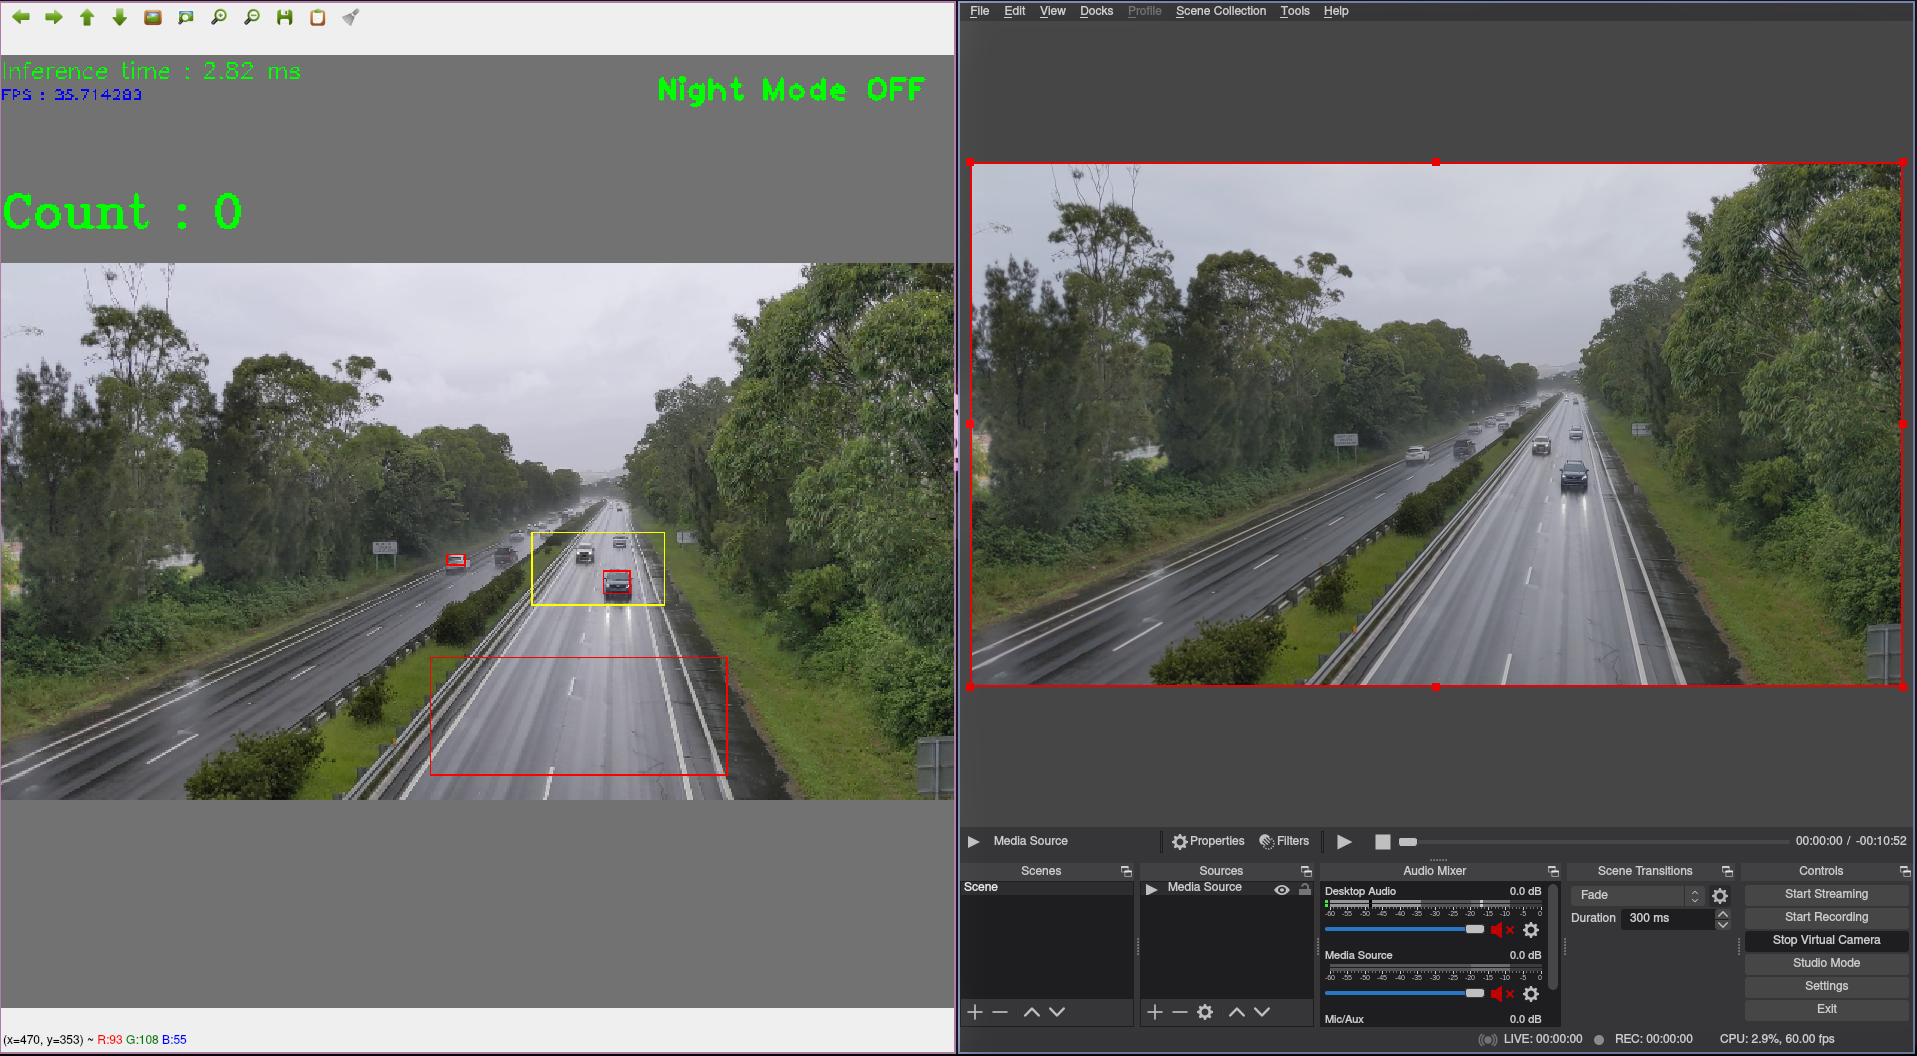
\includegraphics[width=\textwidth]{figures/exp_sim_obs.png}
    \end{center}
    \caption{Experiment Simulation}
    \label{fig:exp_sim_obs}
\end{figure}

\begin{listing}[htbp]
    \centering
\definecolor{bg}{rgb}{0.95,0.95,0.95}
\begin{minted}[
frame=lines,
framesep=2mm,
baselinestretch=1.1,
fontsize=\footnotesize,
bgcolor=bg,
linenos,
]{c++}
#include <opencv2/core.hpp>

VideoCapture cap("test_video/test_video.mp4");
Mat frame;
while(cap.empty() != true){
    cap >> frame;
   
    imshow("My Video", frame);
    waitKey(1);

/*
Actual Video Duration : 10.9803 mins
Total Time Taken : 9.215221 mins
Extra Time Taken : -1.765072 mins
*/
\end{minted}
\caption{OpenCV reading frames faster than actual time}
\label{lst:experiment}
\end{listing}

This project investigates the accuracy of vehicle counting using two variations of YOLOv5 and SORT
algorithm.
This project also investigates the accuracy of nighttime vehicle counting.
The parameters used for obtaining measurements are shown in Tab. \ref{tab:exprunparam}.
Width and height corresponds to the width and height of the region of interest for detection.
X and Y are the top left coordinates of each region of interest.

\begin{table}[htbp]
    \centering
    \begin{adjustbox}{width=1\textwidth}
    \begin{tabular}{c|cccc|cccc|}
    \cline{2-9}
    \textbf{} & \multicolumn{4}{c|}{\textbf{ROI A}} & \multicolumn{4}{c|}{\textbf{ROI B}} \\ \hline
    \multicolumn{1}{|c|}{\textbf{Video Name}} & \multicolumn{1}{c|}{Width} & \multicolumn{1}{c|}{Height} & \multicolumn{1}{c|}{X} & Y & \multicolumn{1}{c|}{Width} & \multicolumn{1}{c|}{Height} & \multicolumn{1}{c|}{X} & Y \\ \hline
    \multicolumn{1}{|c|}{\textbf{test\_video}} & \multicolumn{1}{c|}{640} & \multicolumn{1}{c|}{100} & \multicolumn{1}{c|}{0} & 0 & \multicolumn{1}{c|}{640} & \multicolumn{1}{c|}{100} & \multicolumn{1}{c|}{0} & 350 \\ \hline
    \multicolumn{1}{|c|}{\textbf{rain\_high\_angle}} & \multicolumn{1}{c|}{90} & \multicolumn{1}{c|}{50} & \multicolumn{1}{c|}{356} & 320 & \multicolumn{1}{c|}{200} & \multicolumn{1}{c|}{80} & \multicolumn{1}{c|}{288} & 404 \\ \hline
    \multicolumn{1}{|c|}{\textbf{night\_high\_angle}} & \multicolumn{1}{c|}{250} & \multicolumn{1}{c|}{50} & \multicolumn{1}{c|}{200} & 400 & \multicolumn{1}{c|}{300} & \multicolumn{1}{c|}{60} & \multicolumn{1}{c|}{190} & 454 \\ \hline
    \multicolumn{1}{|c|}{\textbf{night\_high\_angle\_low\_exposure}} & \multicolumn{1}{c|}{250} & \multicolumn{1}{c|}{50} & \multicolumn{1}{c|}{200} & 400 & \multicolumn{1}{c|}{300} & \multicolumn{1}{c|}{60} & \multicolumn{1}{c|}{190} & 454 \\ \hline
    \end{tabular}
    \end{adjustbox}
    \caption{Program Parameters}
    \label{tab:exprunparam}
\end{table}

\chapter{Results and Analysis}
This chapter presents the results of the experiment conducted for the project.
The performance of the application is evaluated in terms of accuracy and average frames per second.
In this case, the accuracy of count is calculated as shown in Eqn. \ref{eq:accuracy}.
The average frames per second was obtained using the Chrono high resolution clock module.

\begin{equation}
    \text{Accuracy (\%)} = \Big(1 - \frac{\lvert\text{Actual Count} - \text{Program
    Count}\rvert}{\text{Actual Count}}\Big)
    \times 100
    \label{eq:accuracy}
\end{equation}

\section{test\_video}

The results for the experiment conducted in daytime with the video from Princes Highway is shown in
Tab. \ref{tab:result_test_video}.
In this experiment, YOLOv5l demonstrates the highest count accuracy at $99.163\%$.
Next, YOLOv5m shows a $0.418\%$ decrease in count accuracy and a $7.466$ increase in FPS when compared
to YOLOv5l.
Furthermore, YOLOv5n and YOLOv5s demonstrates a $1.255\%$ and $0.837\%$ decrease in count accuracy when
compared to YOLOv5l.
This is because YOLOv5l has the most complex detection network as compared to the other variants
tested in the experiments.
The experiment using traditional image processing results in the lowest count accuracy at
$60.669\%$ and an FPS of $90.909$.
This is because traditional image processing is unable to properly differentiate objects which are
close together.
When morphological filtering is used on the frames, close objects will blend together.
Moreover, YOLOv5l has the deepest and widest neural network architecture.
A deeper and wider architecture increases complexity and incurs a higher processing cost.
However, this enables object detection to be more accurate.
This experiment demonstrates that when objects in a video are large, a more complex neural network
can result in a higher count accuracy.

\begin{table}[htbp]
    \centering
    \begin{adjustbox}{width=1\textwidth}
    \begin{tabular}{|c|c|c|c|c|c|c|}
    \hline
    \textbf{Video Name} & \textbf{Model} & \textbf{Actual Count} & \textbf{Program Count} & \textbf{Accuracy (\%)} & \textbf{FPS} & \textbf{Inference Time (ms)} \\ \hline
    \multirow{5}{*}{\textbf{test\_video}} & None & 239 & 145 & 60.669 & 90.909 & 2.737 \\ \cline{2-7}
     & YOLOv5n & 239 & 234 & 97.908 & 47.619 & 1.894 \\ \cline{2-7}
     & YOLOv5s & 239 & 243 & 98.326 & 31.250 & 2.246 \\ \cline{2-7}
     & YOLOv5m & 239 & 242 & 98.745 & 19.231 & 2.797 \\ \cline{2-7}
     & YOLOv5l & 239 & 241 & 99.163 & 11.765 & 3.622 \\ \hline
    \end{tabular}
    \end{adjustbox}
    \caption{Experiment Results: test\_video}
    \label{tab:result_test_video}
\end{table}

\section{rain\_high\_angle}

The results from the experiment conducted at Memorial Drive during daytime is shown in Tab.
\ref{tab:result_rha}.
The experiment rain\_high\_angle shows that YOLOv5m performs the best in terms of count accuracy.
The YOLOv5n and YOLOv5s models demonstrate a $0.543\%$ and $0.272\%$ decrease in count accuracy compared to
YOLOv5m.
In this experiment, YOLOv5l has a lower count accuracy as compared to all other YOLOv5 variants.
This is because YOLOv5l requires high processing power.
In this case, the slow processing of using YOLOv5l results in objects being missed and tracked as
new objects.
This is demonstrated as program counts are higher when using the YOLOv5l model.
Traditional image processing demonstrates a $93.478\%$ accuracy count and the highest FPS at
$90.909$ compared to the other models.
This is because traditional image processing can better differentiate objects which are further
apart.
Camera position tuning can enable the application to perform better using traditional image
processing.

\begin{table}[htbp]
    \begin{adjustbox}{width=1\textwidth}
    \begin{tabular}{|c|c|c|c|c|c|c|}
    \hline
    \textbf{Video Name} & \textbf{Model} & \textbf{Actual Count} & \textbf{Program Count} & \textbf{Accuracy (\%)} & \textbf{FPS} & \textbf{Inference Time (ms)} \\ \hline
    \multirow{5}{*}{\textbf{rain\_high\_angle}} & None & 368 & 392 & 93.478 & 90.909 & 2.489 \\ \cline{2-7}
     & YOLOv5n & 368 & 366 & 99.457 & 47.619 & 2.104 \\ \cline{2-7}
     & YOLOv5s & 368 & 367 & 99.728 & 28.571 & 2.040 \\ \cline{2-7}
     & YOLOv5m & 368 & 368 & 100.000 & 19.608 & 2.749 \\ \cline{2-7}
     & YOLOv5l & 368 & 372 & 98.913 & 11.364 & 3.356 \\ \hline
    \end{tabular}
    \end{adjustbox}
    \caption{Experiment Results: rain\_high\_angle}
    \label{tab:result_rha}
\end{table}

\section{night\_high\_angle}

This experiment is conducted at Memorial Drive during nighttime.
The results from this experiment is shown in Tab. \ref{tab:result_nha}.
This experiment night\_high\_angle demonstrates that traditional image processing performs the best
in terms of count accuracy and FPS at $72.381\%$ and $90.909$ respectively.
Moreover, YOLOv5n and YOLOv5l shows a low count accuracy at $3.810\%$ and $34.286\%$ respectively.
The deep learning detection method did not show a satisfactory performance.
This is because low light eliminates the features which deep learning detection methods need to
differentiate between objects.
In this experiment, the deep learning detection methods show similar processing costs when compared
to the previous experiments.

\begin{table}[htbp]
    \centering
    \begin{adjustbox}{width=1\textwidth}
    \begin{tabular}{|c|c|c|c|c|c|c|}
    \hline
    \textbf{Video Name} & \textbf{Model} & \textbf{Actual Count} & \textbf{Program Count} & \textbf{Accuracy (\%)} & \textbf{FPS} & \textbf{Inference Time (ms)} \\ \hline
     & Night Mode & 105 & 76 & 72.381 & 90.909 & 0.684 \\ \cline{2-7}
    \textbf{night\_high\_angle} & YOLOv5n & 105 & 4 & 3.810 & 41.667 & 2.030 \\ \cline{2-7}
     & YOLOv5l & 105 & 36 & 34.286 & 11.628 & 3.402 \\ \hline
    \end{tabular}
    \end{adjustbox}
\caption{Experiment Results: night\_high\_angle}
\label{tab:result_nha}
\end{table}

\section{night\_high\_angle\_low\_exposure}

This experiment is conducted at Memorial Drive during nighttime.
In this experiment, the camera is set to the lowest possible exposure.
The results of this experiment is reported in Tab. \ref{tab:result_nha_low_exp}.
Traditional image processing demonstrates the highest count accuracy and FPS at $96.040\%$ and
$90.909$ respectively.
Next, YOLOv5n and YOLOv5l reports a count accuracy of $0.990\%$ and $8.911\%$ respectively.
This is because low exposure removes key features from frames which deep learning detection methods
need to identify objects.

\begin{table}[htbp]
    \begin{adjustbox}{width=1\textwidth}
    \begin{tabular}{|c|c|c|c|c|c|c|}
    \hline
    \textbf{Video Name} & \textbf{Model} & \textbf{Actual Count} & \textbf{Program Count} & \textbf{Accuracy (\%)} & \textbf{FPS} & \textbf{Inference Time (ms)} \\ \hline
    \textbf{night\_high\_angle} & Night Mode & 101 & 105 & 96.040 & 90.909 & 0.684 \\ \cline{2-7}
    \textbf{\_low\_exposure} & YOLOv5n & 101 & 1 & 0.990 & 41.667 & 2.044 \\ \cline{2-7}
    & YOLOv5l & 101 & 9 & 8.911 & 10.870 & 3.387 \\ \hline
    \end{tabular}
    \end{adjustbox}
    \caption{Experiment Results: night\_high\_angle\_low\_exposure}
    \label{tab:result_nha_low_exp}
\end{table}

\chapter{Conclusion and Future Work}

In conclusion, deep learning can be used to detect objects during daytime.
This is demonstrated in the experiments test\_video and rain\_high\_angle.
However, deep learning object detection methods can only demonstrate high accuracy when the
lighting conditions in a video is good.
This is because deep learning detections methods need features to identify objects in a frame.
Low lighting conditions remove details in a video frame.
Moreover, convolution neural networks can be used to detect objects in real-time.
This is shown in the experiments where all YOLOv5 models demonstrate an accuracy higher than
$97.908\%$.
In addition, the experiments show that the performance of object counting can be sustained at low FPS.
In this case, the accuracy of vehicle counting only decreases when FPS drops below $11.364\%$.
Next, traditional image processing can be used to detect vehicles when there is video lighting is
low.
This is demonstrated in the experiments night\_high\_angle and night\_high\_angle\_low\_exposure.
In the experiments, traditional image processing using headlight pairing reports an accuracy of
$72.381\%$ and $96.040\%$ respectively.
The two experiments during nighttime demonstrates that the accuracy of nighttime detection is higher
when the exposure is low.
This is due to morphological filtering and headlight pairing benefits from a lower number of details
in frames.

A future research direction is to estimate the location and speed of a vehicle on a 2-D map.
Next, alternate daytime to nighttime switching methods can be identified to reduce false positives
and processing overhead.
Moreover, the tracking algorithm can also be refined with more state-of the art algorithms to
improve object tracking when occlusion is present in a frame.
Furthermore, the application can also be deployed as a supporting library for an android application
for practical testing.
Finally, future works can also consider dynamic vehicle counting in any locations which do not
require any prior setup.


\addcontentsline{toc}{chapter}{Bibliography}
\bibliographystyle{unsrtnat}
\bibliography{references}{}

\clearpage
\appendix
\chapter{Command Line Arguments}

\begin{listing}[htbp]
\definecolor{bg}{rgb}{0.95,0.95,0.95}
\begin{minted}[
frame=lines,
framesep=2mm,
baselinestretch=1,
fontsize=\footnotesize,
bgcolor=bg,
linenos,
]{man}
$ ./build/realtime-counting --help

General Options:
  --help                                Print this help

Required Options:
  --model_path arg (=./dnn_files/yolov5n-opt.onnx)
                                        Deep Learning Model
  --class_path arg (=./dnn_files/coco_c.names)
                                        Class Names
  --model_size arg (=640)               Model Size
  --actual_count arg (=239)             Actual Car Count
  --roi_A arg (={640,100,0,0})          Width, Height and Coordinates
                                        of Region of Interest A
  --roi_B arg (={640,100,0,350})        Width, Height and Coordinates
                                        of Region of Interest B
  --night_mode arg (=0)                 Night Mode Toggle
  --night_roi_1 arg (={20,20,0,0})      Region of Interest 1 to for
                                        Night Automation
  --night_roi_2 arg (={20,20,620,340})  Region of Interest 2 to for
                                        Night Automation
  --preview arg (=0)                    Preview Mode
  --traditional arg (=0)                Traditional Image Processing Mode

\end{minted}
\caption{Command Line Arguments}
\label{lst:cla}
\end{listing}

\end{document}
